\documentclass[conference]{IEEEtran}
\IEEEoverridecommandlockouts
\usepackage{cite}
\usepackage{amsmath,amssymb,amsfonts}
\usepackage{algorithmic}
\usepackage{graphicx}
\usepackage{textcomp}
\usepackage{xcolor}
\usepackage{pifont}
\usepackage{booktabs}
\usepackage{array}
\usepackage{multirow}
% Tighter float parameters to reduce white space
\renewcommand{\topfraction}{0.95}
\renewcommand{\bottomfraction}{0.95}
\renewcommand{\textfraction}{0.05}
\renewcommand{\floatpagefraction}{0.90}
\setcounter{topnumber}{4}
\setcounter{bottomnumber}{4}
\setcounter{totalnumber}{6}
\def\BibTeX{{\rm B\kern-.05em{\sc i\kern-.025em b}\kern-.08em
    T\kern-.1667em\lower.7ex\hbox{E}\kern-.125emX}}
\usepackage{stfloats}
\usepackage{float}
\usepackage{placeins}
\begin{document}

\title{Overcoming Session Drift and Filter Blindness in Motor Imagery BCI: A Multi-Band Space-First CNN with Euclidean Alignment}

\author{
  \IEEEauthorblockN{Satyam Deo}
  \IEEEauthorblockA{\textit{Computer Science and Engineering} \\
  \textit{Indian Institute of Information Technology}\\
  Nagpur, India \\
  bt23csd004@iiitn.ac.in}
  \and
  \IEEEauthorblockN{Dr. Nileshchandra Pikle}
  \IEEEauthorblockA{\textit{Computer Science and Engineering} \\
  \textit{Indian Institute of Information Technology}\\
  Nagpur, India \\
  npikle@iiitn.ac.in}
  \and
  \IEEEauthorblockN{Rajdeep Banerjee}
  \IEEEauthorblockA{\textit{Computer Science and Engineering} \\
  \textit{Indian Institute of Information Technology}\\
  Nagpur, India \\
  bt23csd029@iiitn.ac.in}
  \and
  \IEEEauthorblockN{Abhinav R. Jha}
  \IEEEauthorblockA{\textit{Computer Science and Engineering} \\
  \textit{Indian Institute of Information Technology}\\
  Nagpur, India \\
  bt23csd053@iiitn.ac.in}
}

\maketitle

% -------------------------------------------------------
% ABSTRACT — revised to claim adaptive screening as contribution
% -------------------------------------------------------
\begin{abstract}
Reliable cross-session Motor Imagery Brain--Computer Interface (MI-BCI) decoding remains a challenging problem due to two key factors: session drift, which causes shifts in EEG spatial covariance across recording days, and filter blindness, where broadband processing obscures subject-specific discriminative rhythms. Existing methods such as SWCNet achieve strong within-session performance but degrade significantly under cross-session evaluation.

We propose Multi-Band SWCNet (MB-SWCNet), which extends the Space-First CNN architecture with three components: (1) Euclidean Alignment (EA) to reduce inter-session covariance shift without requiring labeled target data, (2) multi-band decomposition into broadband, mu, and beta frequency bands to enhance discriminative feature extraction, and (3) an ensemble training strategy combining sliding-window augmentation, label smoothing, and soft voting.

The method is evaluated on three benchmark datasets of increasing complexity: BCIC-IV-2a, High Gamma Dataset (HGD), and OpenBMI. MB-SWCNet consistently improves performance over SWCNet in both single-session and cross-session settings, with the largest gains observed on high-density datasets.

Further analysis shows that multi-band features provide stronger class separability than broadband signals, while Euclidean Alignment is particularly beneficial for subjects with high inter-session variability. We identify Stable-Manifold Subjects---a physiologically distinct subpopulation for whom EA is counterproductive---and propose a two-criterion pre-session screening rule to adaptively select the preprocessing strategy per individual.
\end{abstract}

\begin{IEEEkeywords}
Brain--Computer Interface, Motor Imagery, EEG, Euclidean Alignment, Multi-Band Filtering, Convolutional Neural Network, Session Drift, Filter Blindness, Subject-Dependent
\end{IEEEkeywords}

% -------------------------------------------------------
\section{Introduction}
% -------------------------------------------------------

Brain--Computer Interfaces (BCIs) provide a direct communication pathway between the human brain and external devices, serving as a transformative technology for neurorehabilitation and assistive systems. By sensing and decoding brain activity, BCIs empower individuals with severe motor disabilities to control prosthetics, robotic wheelchairs, and communication interfaces without relying on peripheral nerves or muscles \cite{b2}. Among various non-invasive neuroimaging modalities, Electroencephalography (EEG) has emerged as the most widely adopted method due to its high temporal resolution, portability, and cost-effectiveness \cite{b3}. In a typical Motor Imagery BCI (MI-BCI) system, an individual imagines performing a specific motor action (e.g., moving the right hand or both feet), and the resulting neurophysiological changes captured by scalp electrodes are translated into digital command signals by a decoding algorithm.

Despite significant advancements in neurotechnology, the practical deployment of MI-BCI systems outside controlled laboratory calibration sessions remains limited. The core bottleneck is the inherently low Signal-to-Noise Ratio (SNR) of EEG data, compounded by environmental artifacts and biological non-stationarity \cite{b4}. In particular, real-world MI-BCI decoding is affected by two persistent and technically distinct challenges.

\textbf{Session Drift} refers to the spatial variability of EEG signals across different recording sessions. Between a calibration session (Day 1) and a deployment session (Day 2), changes in electrode placement, skin impedance, and underlying neural activity alter the spatial covariance structure of the data. As a result, models trained on Session 1 often experience significant performance degradation when evaluated on Session 2.

\textbf{Filter Blindness} arises when decoding models rely on fixed broadband filtering (typically 4--40 Hz). Motor imagery is primarily characterized by Event-Related Desynchronization and Synchronization (ERD/ERS) in the Mu (8--13 Hz) and Beta (13--30 Hz) bands \cite{b5}. Since these patterns vary across subjects, broadband representations can obscure discriminative frequency-specific information, limiting classification performance.

Traditionally, machine learning approaches such as Common Spatial Patterns (CSP) and Support Vector Machines (SVMs) have been used to extract and classify ERD/ERS features. More recently, deep learning methods, particularly Convolutional Neural Networks (CNNs), have become the dominant paradigm for MI-EEG decoding \cite{b6,b7}. Singh et al. introduced SWCNet \cite{b1}, a Space-First CNN architecture combined with sliding-window augmentation, achieving strong performance in single-session evaluations. However, its performance drops substantially under cross-session conditions due to the absence of mechanisms to handle distributional shifts.

To evaluate such scenarios, two commonly used protocols are considered. \textbf{Setup I (single-session)} involves training and testing on data drawn from the same distribution, typically by mixing sessions. In contrast, \textbf{Setup II (cross-session)} trains the model on Session 1 and evaluates it on Session 2, reflecting real-world deployment conditions where no labeled target-session data is available.

Motivated by these limitations, we propose Multi-Band SWCNet (MB-SWCNet), which extends the Space-First architecture with targeted improvements to enhance cross-session robustness and frequency-specific feature extraction. The key contributions of this work are summarized as follows:

\begin{itemize}
    \item \textbf{Euclidean Alignment (EA):} An unsupervised alignment technique that reduces inter-session covariance differences without requiring labeled target data.
    \item \textbf{Multi-Band Spatial-Frequency Expansion:} Decomposition of EEG signals into broadband, Mu, and Beta bands to capture subject-specific discriminative patterns.
    \item \textbf{Ensemble Training Strategy:} A combination of sliding-window augmentation, label smoothing, and soft-voting to improve generalization.
    \item \textbf{Comprehensive Evaluation:} Validation on three benchmark datasets (BCIC-IV-2a, HGD, OpenBMI) under both Setup I and Setup II protocols.
    \item \textbf{Adaptive Screening Rule:} A two-criterion pre-session heuristic that identifies Stable-Manifold Subjects from Session~1 data alone and selectively disables EA for individuals whose neural manifold does not require correction.
    \item \textbf{Mechanistic Insights:} Analysis of when and why the proposed components are effective, including identification of subject-specific variability patterns.
\end{itemize}

The remainder of this paper is organized as follows. Section II reviews related work in MI-EEG decoding and domain adaptation. Section III describes the proposed methodology, including Euclidean Alignment and multi-band expansion. Section IV presents the experimental setup and results. Section V provides mechanistic analysis and ablation studies. Finally, Section VI concludes the paper and outlines future research directions.

% -------------------------------------------------------
\section{Related Work}
% -------------------------------------------------------

Research on improving Motor Imagery Brain--Computer Interface (MI-BCI) decoding has evolved from classical signal processing approaches to modern deep learning frameworks. Early methods relied on handcrafted feature extraction techniques combined with traditional machine learning classifiers. Common Spatial Patterns (CSP) \cite{b8} and its extension Filter Bank CSP (FBCSP) \cite{b9} were widely used to enhance class separability by maximizing variance differences across spatial channels. These methods, typically coupled with Linear Discriminant Analysis (LDA) or Support Vector Machines (SVMs), perform well in controlled single-session settings. However, they are sensitive to noise, require careful feature engineering, and often fail to generalize under non-stationary conditions such as cross-session scenarios.

With the advancement of deep learning, Convolutional Neural Networks (CNNs) have become the dominant paradigm for MI-EEG decoding due to their ability to automatically learn spatial-temporal representations. EEGNet \cite{b10} introduced a compact and generalizable architecture suitable for multiple EEG paradigms. ShallowConvNet and DeepConvNet \cite{b9} further demonstrated that space-first convolutional structures are effective in capturing spatial dependencies across electrodes, particularly in high-density EEG data. Subsequent works have explored multi-scale and hybrid CNN architectures \cite{b15}, improving feature richness and robustness. Despite these advantages, CNN-based models are typically trained under the assumption of data stationarity and often rely on broadband inputs, limiting their ability to capture subject-specific frequency characteristics.

To model temporal dependencies more effectively, sequence-based architectures such as Long Short-Term Memory (LSTM) networks \cite{b11} and hybrid CNN-LSTM models \cite{b12,b13} have been proposed. These models enhance temporal representation but introduce higher computational complexity and training instability. Attention-based models such as ATCNet \cite{b14} further improve temporal modeling through adaptive weighting mechanisms, achieving promising results in subject-independent settings. However, these approaches still struggle with distributional shifts across sessions, which remain a major challenge in real-world deployment.

SWCNet \cite{b1} represents a recent advancement, introducing a Space-First CNN architecture combined with sliding-window augmentation. By prioritizing spatial feature extraction, it achieves strong subject-dependent performance across multiple datasets. Nevertheless, it assumes consistency between training and testing distributions and relies on broadband representations, making it vulnerable to session drift and limited in capturing frequency-specific discriminative patterns.

In parallel, domain adaptation techniques have been explored to address EEG non-stationarity. Riemannian geometry-based methods, such as Euclidean Alignment (EA) \cite{b16}, align covariance matrices in a shared space without requiring labeled target data. While these approaches provide a principled solution to distributional shift, they are primarily studied in cross-subject settings and are less explored in strict cross-session scenarios. Other methods, including adversarial domain adaptation and transfer learning, aim to learn invariant representations but often require complex training procedures or partial access to target-domain information.

Table~\ref{tab:sota} summarizes representative approaches and highlights key limitations. While classical methods offer interpretability and simplicity, and deep learning models provide strong representation learning capabilities, existing approaches do not simultaneously address both cross-session covariance shift and subject-specific frequency modeling under strict cross-session evaluation protocols.

% -------------------------------------------------------
% TABLE I — added FBCSP row as separate entry; MB-SWCNet is only method
% addressing both drift and multi-band simultaneously
% -------------------------------------------------------
\begin{table*}[t]
\caption{Overview of State-of-the-Art Models in MI-EEG Classification}
\begin{center}
\setlength{\tabcolsep}{5pt}
\begin{tabular}{|l|l|l|c|c|}
\hline
\textbf{Study} & \textbf{Approach} & \textbf{Key Strength} & \textbf{Handles Drift} & \textbf{Multi-Band} \\
\hline
Blankertz et al. \cite{b8} & CSP + LDA & Interpretable spatial filters & No & No \\
\hline
Ang et al. \cite{b9} & FBCSP + SVM & Frequency-specific spatial filtering & No & Yes \\
\hline
Schirrmeister et al. \cite{b9} & Shallow/Deep ConvNet & Strong spatial modeling & No & No \\
\hline
Lawhern et al. \cite{b10} & EEGNet & Compact and generalizable & No & No \\
\hline
Wang et al. \cite{b11} & LSTM & Temporal dependency modeling & No & No \\
\hline
Zhang et al. \cite{b12} & CNN + LSTM & Spatial-temporal fusion & No & No \\
\hline
Altaheri et al. \cite{b14} & ATCNet & Attention-based temporal learning & No & No \\
\hline
Singh et al. \cite{b1} & SWCNet & Space-first CNN + augmentation & No & No \\
\hline
\textbf{MB-SWCNet (Ours)} & \textbf{EA + Multi-Band + Ensemble} & \textbf{Alignment + multi-band + ensemble} & \textbf{Yes} & \textbf{Yes} \\
\hline
\end{tabular}
\label{tab:sota}
\end{center}
\end{table*}

This gap motivates the development of a unified framework that integrates domain alignment with frequency-specific feature extraction to improve robustness in cross-session MI-BCI decoding.

% -------------------------------------------------------
\section{Proposed Methodology}
% -------------------------------------------------------

To address the challenges of Session Drift and Filter Blindness in cross-session MI-BCI decoding, the proposed framework (MB-SWCNet) extends the Space-First convolutional paradigm with domain alignment, multi-band feature expansion, and an ensemble-based prediction strategy.

\subsection{Datasets}

Table~\ref{tab:datasets} summarises the datasets used to evaluate the proposed model across varying spatial resolutions and population scales.

\begin{table}[t]
\caption{Overview of Datasets Used}
\begin{center}
\begin{tabular}{|l|c|c|c|c|c|}
\hline
\textbf{Dataset} & \textbf{Subj.} & \textbf{Sess.} & \textbf{Chan.} & \textbf{Classes} & \textbf{Trials/Subj.} \\
\hline
BCIC-IV-2a \cite{b17} & 9 & 2 & 22 & 4 & 288 \\
\hline
HGD \cite{b9} & 14 & 2 & 44 & 4 & $\sim$1000 \\
\hline
OpenBMI \cite{b18} & 54 & 2 & 62 & 2 & 100 \\
\hline
\end{tabular}
\label{tab:datasets}
\end{center}
\end{table}

All signals are resampled to a common frequency of $F_s = 250$ Hz, where $F_s$ denotes the sampling frequency. The electrode selection for OpenBMI retains the full 62-channel configuration rather than the 20-channel motor subset used in the original SWCNet evaluation. This choice is motivated by the hypothesis that higher spatial resolution provides richer covariance structure for Euclidean Alignment and greater spatial-frequency diversity for the $(3C,\,1)$ kernel. Consequently, direct numerical comparison with SWCNet on OpenBMI reflects both architectural and preprocessing differences and should be interpreted accordingly; the BCIC-IV-2a and HGD comparisons, which use matched electrode configurations, provide the controlled basis for performance attribution.

\subsection{Pipeline Formulation}

The complete processing pipeline is defined as:

\begin{equation}
\hat{y} = \mathcal{E} \Big( f_{\theta} \big( \mathcal{W} ( \mathcal{B} ( \mathcal{A}(X) ) ) \big) \Big)
\end{equation}

where $X \in \mathbb{R}^{C \times T_{raw}}$ denotes the raw EEG trial, $C$ is the number of EEG channels, and $T_{raw}$ is the number of temporal samples per trial. $\mathcal{A}(\cdot)$ represents Euclidean Alignment, $\mathcal{B}(\cdot)$ denotes multi-band decomposition, $\mathcal{W}(\cdot)$ denotes sliding-window segmentation, $f_{\theta}(\cdot)$ is the convolutional neural network parameterized by $\theta$, $\mathcal{E}(\cdot)$ denotes ensemble aggregation, and $\hat{y}$ is the predicted class label.

\subsection{Unsupervised Domain Adaptation: Euclidean Alignment}

Let $X_i \in \mathbb{R}^{C \times T_{raw}}$ denote the $i$-th EEG trial, where $i = 1,2,\dots,N$ indexes the trials and $N$ is the total number of trials.

The reference covariance matrix $\bar{R} \in \mathbb{R}^{C \times C}$ is computed as:

\begin{equation}
\bar{R} = \frac{1}{N} \sum_{i=1}^{N} \frac{X_i X_i^T}{T_{raw}}
\end{equation}

where $(\cdot)^T$ denotes the transpose operator.

The alignment matrix $M \in \mathbb{R}^{C \times C}$ is defined as:

\begin{equation}
M = \bar{R}^{-1/2}
\end{equation}

where $\bar{R}^{-1/2}$ denotes the inverse square root of the covariance matrix.

Each trial is transformed as:

\begin{equation}
\tilde{X}_i = M X_i
\end{equation}

where $\tilde{X}_i \in \mathbb{R}^{C \times T_{raw}}$ represents the aligned EEG trial. Euclidean Alignment is applied independently to each session using only that session's own trials to compute the reference covariance matrix. For the training session, the alignment is derived from training trials exclusively. For the test session, it is computed from all available test-session trials prior to inference, requiring no label information whatsoever. This design ensures strict separation between sessions and eliminates any possibility of data leakage.

\subsection{Multi-Band Spatial-Frequency Expansion}

Each aligned trial $\tilde{X}_i$ is decomposed into multiple frequency components using bandpass filters.

The filtered signals are denoted as:
\begin{itemize}
    \item $\tilde{X}_i^{broad} \in \mathbb{R}^{C \times T_{raw}}$: broadband signal (4--40 Hz)
    \item $\tilde{X}_i^{mu} \in \mathbb{R}^{C \times T_{raw}}$: Mu band (8--13 Hz)
    \item $\tilde{X}_i^{beta} \in \mathbb{R}^{C \times T_{raw}}$: Beta band (13--30 Hz)
\end{itemize}

These components are concatenated along the channel dimension:

\begin{equation}
\tilde{X}_i^{mb} = \text{concat} \left( \tilde{X}_i^{broad}, \tilde{X}_i^{mu}, \tilde{X}_i^{beta} \right)
\end{equation}

where $\tilde{X}_i^{mb} \in \mathbb{R}^{3C \times T_{raw}}$ and $\text{concat}(\cdot)$ denotes channel-wise concatenation.

\subsection{Architecture: Multi-Band SWCNet}

\begin{figure*}[t]
\centerline{\includegraphics[width=\textwidth]{fig1.png}}
\caption{Processing pipeline: EEG $\rightarrow$ Euclidean Alignment $\rightarrow$ Multi-Band Expansion $\rightarrow$ Sliding Window $\rightarrow$ CNN Ensemble $\rightarrow$ Prediction}
\label{fig:arch_diag}
\end{figure*}

\noindent \textit{1) Sliding Window Segmentation:} Each trial is segmented into overlapping windows of length $T_{win} = 750$ samples, where $T_{win}$ denotes the number of samples per window.

\vspace{1ex}
\noindent \textit{2) Space-First Convolution:} A convolutional kernel of size $(3C,1)$ performs spatial filtering across all channels. By receiving the concatenated three-band input, this kernel is mathematically forced to learn optimal cross-band spatial weightings per subject, effectively acting as a subject-specific frequency selector without any explicit mechanism to do so.

\begin{table}[t]
\caption{Parameters of the MB-SWCNet Architecture}
\begin{center}
\setlength{\tabcolsep}{3pt}
\small
\begin{tabular}{|l|c|c|l|}
\hline
\textbf{Layer} & \textbf{Filt.} & \textbf{Kernel} & \textbf{Details} \\
\hline
Input          & ---  & $(3C, T_{win})$ & Multi-band input \\
\hline
Spatial Conv2D & 8    & $(3C, 1)$       & ReLU + BN \\
\hline
Temporal Conv2D& 16   & $(1, 64)$       & ReLU + BN \\
\hline
Avg Pooling    & ---  & $(1, 2)$        & Stride 2 \\
\hline
Pointwise Conv2D& 8   & $(1, 1)$        & ReLU + BN \\
\hline
Avg Pooling    & ---  & $(1, 4)$        & Stride 4 \\
\hline
Avg Pooling    & ---  & $(1, 8)$        & Stride 8 \\
\hline
Dropout        & ---  & ---             & rate $= 0.5$ \\
\hline
Dense          & $K$  & ---             & Softmax; $K$ classes \\
\hline
\end{tabular}
\label{tab:params}
\end{center}
\end{table}

\vspace{1ex}
\noindent \textit{3) Ensemble Prediction:} The final prediction is computed as:

\begin{equation}
\hat{y} = \arg\max_{k} \frac{1}{S} \sum_{s=1}^{S} p_k^{(s)}
\end{equation}

where $p_k^{(s)}$ denotes the predicted probability for class $k$ from the $s$-th prediction, $k \in \{1, \dots, K\}$ indexes the classes, and $S$ is the total number of predictions aggregated across windows and models. The ensemble size of $S = 5$ models was selected based on validation variance stabilization observed beyond 5 folds in 10-fold cross-validation. Label smoothing with $\epsilon = 0.1$ follows standard practice for multi-class problems with soft targets, where values in the range 0.05--0.15 consistently provide regularization without degrading probability calibration. Both values were fixed prior to final evaluation and were not tuned per subject.

% -------------------------------------------------------
\section{Experimental Results}
% -------------------------------------------------------

\subsection{Experimental Setup and Evaluation Protocols}

All experiments are conducted under two strictly defined Subject-Dependent evaluation protocols, which reflect progressively more demanding real-world deployment conditions.

\textbf{Setup I (Single-Session):} Training and test data are drawn from a combined pool of all sessions for each subject and partitioned into training, testing, and validation subsets with a ratio of 50:30:20. Because both sessions contribute to the training pool, the model is exposed to samples from the same distributional regime as the test data. This setup measures peak within-distribution classification capacity and serves as the upper-bound reference for model expressiveness.

\textbf{Setup II (Cross-Session):} Session 1 is used exclusively for training and Session 2 is held out as the entirely unseen test set, with no data leakage between sessions. This protocol directly simulates the real-world constraint where a BCI system is calibrated on Day 1 and deployed on Day 2, making it the primary evaluation of practical cross-session robustness. Within the training session, 10-fold cross-validation is applied to monitor overfitting, with the best checkpoint selected per fold.

All models use: batch size 32, Adam optimiser with initial learning rate 0.001, early stopping patience of 20 epochs, maximum 200 epochs, and dropout rate 0.5. The baseline for all comparisons is SWCNet~\cite{b1}. To assess statistical reliability, per-subject accuracy pairs (SWCNet vs.\ MB-SWCNet) are compared using the Wilcoxon signed-rank test, a non-parametric test appropriate for the small subject counts ($n = 9, 14, 54$) and non-Gaussian accuracy distributions typical of BCI studies.

The Setup~I vs.\ Setup~II gap is itself diagnostic: SWCNet's average accuracy drop from Setup~I to Setup~II ranges from 27.84\% on BCIC-IV-2a to 33.66\% on OpenBMI, quantifying the severity of Session Drift in the absence of domain adaptation. MB-SWCNet substantially closes this gap while also improving Setup~I accuracy---confirming that the proposed novelties are complementary rather than conflicting.

\subsection{BCIC-IV-2a Results}

Table~\ref{tab:bcic_combined} presents per-subject results for both Setup~I and Setup~II on BCIC-IV-2a. Under Setup~I, MB-SWCNet achieves 99.81\% vs.\ SWCNet's 97.42\% (+2.39\%). Under Setup~II, MB-SWCNet achieves 74.00\% vs.\ SWCNet's 69.58\% (+4.41\%, average F1 = 0.7340). Improvements are observed for all 9 subjects under both protocols, demonstrating consistent gains with no subject harmed.

\begin{table*}[t]
\caption{BCIC-IV-2a --- Setup I and Setup II Subject-Dependent Results}
\begin{center}
\setlength{\tabcolsep}{3.5pt}
\begin{tabular}{|c|cc|cc||cc|cc|}
\hline
\multirow{3}{*}{\textbf{Subj.}} &
\multicolumn{4}{c||}{\textbf{Experiment Setup I}} &
\multicolumn{4}{c|}{\textbf{Experiment Setup II}} \\
\cline{2-9}
& \multicolumn{2}{c|}{\textbf{SWCNet \cite{b1}}} & \multicolumn{2}{c||}{\textbf{MB-SWCNet}} &
  \multicolumn{2}{c|}{\textbf{SWCNet \cite{b1}}} & \multicolumn{2}{c|}{\textbf{MB-SWCNet}} \\
\cline{2-9}
& Acc (\%) & F1 & Acc (\%) & F1 & Acc (\%) & F1 & Acc (\%) & F1 \\
\hline
S1 & 98.64 & 0.9864 & 100.00 & 1.0000 & 78.16 & 0.7812 & 86.81 & 0.8683 \\
S2 & 97.36 & 0.9736 & 99.62  & 0.9962 & 50.44 & 0.4712 & 54.17 & 0.5169 \\
S3 & 98.99 & 0.9899 & 99.62  & 0.9962 & 86.81 & 0.8681 & 89.93 & 0.8976 \\
S4 & 97.31 & 0.9731 & 100.00 & 1.0000 & 65.81 & 0.6559 & 71.18 & 0.7096 \\
S5 & 93.03 & 0.9303 & 99.62  & 0.9962 & 53.33 & 0.5077 & 58.68 & 0.5727 \\
S6 & 96.51 & 0.9651 & 99.43  & 0.9943 & 54.96 & 0.5253 & 56.60 & 0.5652 \\
S7 & 98.89 & 0.9889 & 100.00 & 1.0000 & 81.75 & 0.8175 & 83.68 & 0.8329 \\
S8 & 97.89 & 0.9789 & 100.00 & 1.0000 & 79.17 & 0.7917 & 83.33 & 0.8310 \\
S9 & 98.14 & 0.9814 & 100.00 & 1.0000 & 75.83 & 0.7583 & 81.60 & 0.8116 \\
\hline
\textbf{Avg} & \textbf{97.42} & \textbf{0.9742} & \textbf{99.81} & \textbf{0.9981} & \textbf{69.58} & \textbf{0.6909} & \textbf{74.00} & \textbf{0.7340} \\
\hline
\end{tabular}
\label{tab:bcic_combined}
\end{center}
\end{table*}

\subsection{High Gamma Dataset (HGD) Results}

Table~\ref{tab:hgd_combined} presents per-subject results for both setups on HGD. Under Setup~I, MB-SWCNet achieves 99.96\% vs.\ SWCNet's 92.27\% (+7.70\%), with gains up to +30.72\% for S7. Under Setup~II, MB-SWCNet achieves 86.16\% vs.\ SWCNet's 81.81\% (+4.35\%). The Setup~II results reveal a clear bimodal distribution: 9 of 14 subjects show strong gains, while 5 subjects exhibit accuracy decreases under the cross-session protocol---a heterogeneity that motivates the mechanistic analyses in Section~\ref{sec:mechanistic}.

\begin{table*}[t]
\caption{High Gamma Dataset --- Setup I and Setup II Subject-Dependent Results}
\begin{center}
\setlength{\tabcolsep}{3.5pt}
\begin{tabular}{|c|cc|cc||cc|cc|}
\hline
\multirow{3}{*}{\textbf{Subj.}} &
\multicolumn{4}{c||}{\textbf{Experiment Setup I}} &
\multicolumn{4}{c|}{\textbf{Experiment Setup II}} \\
\cline{2-9}
& \multicolumn{2}{c|}{\textbf{SWCNet \cite{b1}}} & \multicolumn{2}{c||}{\textbf{MB-SWCNet}} &
  \multicolumn{2}{c|}{\textbf{SWCNet \cite{b1}}} & \multicolumn{2}{c|}{\textbf{MB-SWCNet}} \\
\cline{2-9}
& Acc (\%) & F1 & Acc (\%) & F1 & Acc (\%) & F1 & Acc (\%) & F1 \\
\hline
S1  & 97.61 & 0.9762 & 100.00 & 1.0000 & 79.29 & 0.7929 & 76.25  & 0.7625 \\
S2  & 81.69 & 0.8204 & 99.78  & 0.9978 & 67.49 & 0.6749 & 86.25  & 0.8625 \\
S3  & 98.75 & 0.9875 & 100.00 & 1.0000 & 95.01 & 0.9501 & 94.38  & 0.9438 \\
S4  & 96.96 & 0.9696 & 100.00 & 1.0000 & 93.37 & 0.9337 & 90.00  & 0.9000 \\
S5  & 97.21 & 0.9721 & 100.00 & 1.0000 & 89.03 & 0.8903 & 68.12  & 0.6812 \\
S6  & 87.49 & 0.8749 & 100.00 & 1.0000 & 87.18 & 0.8718 & 93.12  & 0.9312 \\
S7  & 69.18 & 0.6918 & 99.90  & 0.9990 & 70.00 & 0.7000 & 85.00  & 0.8500 \\
S8  & 96.78 & 0.9678 & 100.00 & 1.0000 & 75.79 & 0.7579 & 93.75  & 0.9375 \\
S9  & 96.79 & 0.9679 & 100.00 & 1.0000 & 91.24 & 0.9124 & 75.62  & 0.7562 \\
S10 & 96.63 & 0.9663 & 99.90  & 0.9989 & 85.55 & 0.8555 & 95.00  & 0.9500 \\
S11 & 78.74 & 0.7874 & 100.00 & 1.0000 & 68.29 & 0.6829 & 70.62  & 0.7062 \\
S12 & 97.92 & 0.9792 & 100.00 & 1.0000 & 89.13 & 0.8913 & 86.88  & 0.8688 \\
S13 & 96.57 & 0.9657 & 100.00 & 1.0000 & 83.54 & 0.8354 & 94.38  & 0.9438 \\
S14 & 99.39 & 0.9939 & 99.90  & 0.9990 & 70.38 & 0.7038 & 96.88  & 0.9688 \\
\hline
\textbf{Avg} & \textbf{92.27} & \textbf{0.9226} & \textbf{99.96} & \textbf{0.9996} & \textbf{81.81} & \textbf{0.8142} & \textbf{86.16} & \textbf{0.8616} \\
\hline
\end{tabular}
\label{tab:hgd_combined}
\end{center}
\end{table*}

\subsection{OpenBMI Results}

Table~\ref{tab:openbmi_combined} presents full per-subject results for both setups on OpenBMI---the most challenging dataset with 54 subjects and 62 high-density electrodes. Under Setup~I, MB-SWCNet achieves 99.50\% vs.\ SWCNet's 90.82\%\footnote{Subject~29 data was corrupted during preprocessing due to a file parsing error in the OpenBMI loader and is excluded from the Setup~I average computation. Setup~II results for S29 are retained as the test session was unaffected. The reported Setup~I average of 99.50\% is therefore computed over 53 valid subjects.}, with 28 subjects reaching exactly 100\%. Under Setup~II, MB-SWCNet achieves 65.18\% vs.\ SWCNet's 57.16\% (+8.03\%)---the largest aggregate margin across all three datasets. Two ``super-responder'' subjects reach 100\% cross-session accuracy: S21 (+49.70\%) and S36 (+40.46\%). The +8.03\% Setup~II improvement completes a clear electrode-density scaling law: +4.41\% (22 channels) $\rightarrow$ +4.35\% (44 channels) $\rightarrow$ +8.03\% (62 channels).

\begin{table*}[t]
\caption{Full OpenBMI Results --- Setup I and Setup II Subject-Dependent Accuracy Comparison}
\begin{center}
\resizebox{\textwidth}{!}{%
\setlength{\tabcolsep}{2.8pt}
\begin{tabular}{|c|cc|cc||cc|cc||c|cc|cc||cc|cc|}
\hline
\multirow{3}{*}{\textbf{S}} &
\multicolumn{4}{c||}{\textbf{Setup I}} &
\multicolumn{4}{c||}{\textbf{Setup II}} &
\multirow{3}{*}{\textbf{S}} &
\multicolumn{4}{c||}{\textbf{Setup I}} &
\multicolumn{4}{c|}{\textbf{Setup II}} \\
\cline{2-9}\cline{11-18}
& \multicolumn{2}{c|}{\textbf{SWCNet}} & \multicolumn{2}{c||}{\textbf{MB}} &
  \multicolumn{2}{c|}{\textbf{SWCNet}} & \multicolumn{2}{c||}{\textbf{MB}} & &
  \multicolumn{2}{c|}{\textbf{SWCNet}} & \multicolumn{2}{c||}{\textbf{MB}} &
  \multicolumn{2}{c|}{\textbf{SWCNet}} & \multicolumn{2}{c|}{\textbf{MB}} \\
\cline{2-9}\cline{11-18}
& Acc & F1 & Acc & F1 & Acc & F1 & Acc & F1 & & Acc & F1 & Acc & F1 & Acc & F1 & Acc & F1 \\
\hline
S1  & 90.80 & 0.9080 & 99.29 & 0.9929 & 47.42 & 0.4662 & 80.00 & 0.8000 &
S28 & 92.58 & 0.9258 & 100.00 & 1.0000 & 66.85 & 0.6650 & 96.00 & 0.9600 \\
S2  & 93.05 & 0.9305 & 100.00 & 1.0000 & 63.55 & 0.6337 & 76.00 & 0.7600 &
S29 & 99.07 & 0.9907 & 99.50* & 0.9950 & 79.94 & 0.7984 & 65.98 & 0.6598 \\
S3  & 87.26 & 0.8725 & 100.00 & 1.0000 & 57.07 & 0.5700 & 79.00 & 0.7900 &
S30 & 90.27 & 0.9027 & 99.52 & 0.9952 & 60.04 & 0.6225 & 50.00 & 0.5000 \\
S4  & 94.20 & 0.9420 & 99.76 & 0.9976 & 72.49 & 0.7239 & 58.00 & 0.5800 &
S31 & 94.13 & 0.9412 & 99.76 & 0.9976 & 62.66 & 0.6225 & 68.00 & 0.6800 \\
S5  & 84.68 & 0.8467 & 100.00 & 1.0000 & 57.89 & 0.5754 & 87.00 & 0.8700 &
S32 & 87.76 & 0.8775 & 100.00 & 1.0000 & 48.94 & 0.4822 & 95.00 & 0.9500 \\
S6  & 97.02 & 0.9702 & 100.00 & 1.0000 & 79.89 & 0.7986 & 84.00 & 0.8400 &
S33 & 88.63 & 0.8863 & 100.00 & 1.0000 & 51.06 & 0.4955 & 84.00 & 0.8400 \\
S7  & 92.39 & 0.9239 & 99.52 & 0.9952 & 59.60 & 0.5955 & 70.00 & 0.7000 &
S34 & 85.18 & 0.8517 & 98.81 & 0.9881 & 51.02 & 0.5079 & 52.00 & 0.5200 \\
S8  & 92.82 & 0.9281 & 100.00 & 1.0000 & 60.16 & 0.6011 & 64.00 & 0.6400 &
S35 & 99.82 & 0.9982 & 99.52 & 0.9952 & 94.82 & 0.9481 & 65.00 & 0.6500 \\
S9  & 82.08 & 0.8204 & 100.00 & 1.0000 & 51.61 & 0.5087 & 65.00 & 0.6500 &
S36 & 92.94 & 0.9294 & 100.00 & 1.0000 & 59.54 & 0.5936 & 100.00 & 1.0000 \\
S10 & 92.73 & 0.9273 & 100.00 & 1.0000 & 47.56 & 0.4731 & 50.00 & 0.5000 &
S37 & 84.49 & 0.8446 & 100.00 & 1.0000 & 52.35 & 0.5088 & 90.00 & 0.9000 \\
S11 & 91.27 & 0.9127 & 99.05 & 0.9905 & 53.19 & 0.5170 & 53.00 & 0.5300 &
S38 & 78.14 & 0.7807 & 99.29 & 0.9929 & 52.76 & 0.5245 & 51.00 & 0.5100 \\
S12 & 89.75 & 0.8974 & 99.76 & 0.9976 & 61.85 & 0.6088 & 63.00 & 0.6300 &
S39 & 92.62 & 0.9262 & 99.05 & 0.9905 & 53.11 & 0.5262 & 76.00 & 0.7600 \\
S13 & 86.67 & 0.8666 & 100.00 & 1.0000 & 53.70 & 0.5296 & 54.00 & 0.5400 &
S40 & 90.32 & 0.9032 & 99.52 & 0.9952 & 54.40 & 0.5129 & 59.00 & 0.5900 \\
S14 & 90.75 & 0.9073 & 100.00 & 1.0000 & 51.57 & 0.5107 & 51.00 & 0.5100 &
S41 & 86.96 & 0.8695 & 98.33 & 0.9833 & 50.83 & 0.5115 & 53.00 & 0.5300 \\
S15 & 95.48 & 0.9547 & 99.76 & 0.9976 & 69.91 & 0.6907 & 50.00 & 0.5000 &
S42 & 97.93 & 0.9770 & 100.00 & 1.0000 & 55.64 & 0.5529 & 60.00 & 0.6000 \\
S16 & 93.85 & 0.9383 & 99.29 & 0.9929 & 60.02 & 0.5980 & 50.00 & 0.5000 &
S43 & 93.99 & 0.9398 & 98.57 & 0.9857 & 60.11 & 0.5896 & 62.00 & 0.6200 \\
S17 & 89.57 & 0.8957 & 99.52 & 0.9952 & 52.44 & 0.5181 & 50.00 & 0.5000 &
S44 & 90.06 & 0.9005 & 100.00 & 1.0000 & 50.12 & 0.5000 & 96.00 & 0.9600 \\
S18 & 87.69 & 0.8768 & 100.00 & 1.0000 & 46.99 & 0.4676 & 84.00 & 0.8400 &
S45 & 90.43 & 0.9043 & 99.76 & 0.9976 & 51.98 & 0.5166 & 85.00 & 0.8500 \\
S19 & 92.80 & 0.9280 & 99.52 & 0.9952 & 51.27 & 0.5181 & 66.00 & 0.6600 &
S46 & 92.75 & 0.9275 & 98.81 & 0.9881 & 56.46 & 0.5589 & 51.00 & 0.5100 \\
S20 & 94.18 & 0.9417 & 99.29 & 0.9929 & 53.49 & 0.5143 & 55.00 & 0.5500 &
S47 & 92.60 & 0.9259 & 99.52 & 0.9952 & 60.23 & 0.6005 & 53.00 & 0.5300 \\
S21 & 92.24 & 0.9223 & 100.00 & 1.0000 & 50.30 & 0.5016 & 100.00 & 1.0000 &
S48 & 93.86 & 0.9385 & 99.52 & 0.9952 & 61.49 & 0.6116 & 66.00 & 0.6600 \\
S22 & 90.69 & 0.9069 & 100.00 & 1.0000 & 50.23 & 0.5000 & 62.00 & 0.6200 &
S49 & 88.76 & 0.8876 & 99.29 & 0.9929 & 55.94 & 0.5460 & 57.00 & 0.5700 \\
S23 & 89.67 & 0.8967 & 100.00 & 1.0000 & 50.76 & 0.4847 & 83.00 & 0.8300 &
S50 & 92.50 & 0.9248 & 98.10 & 0.9810 & 52.17 & 0.5143 & 52.00 & 0.5200 \\
S24 & 88.32 & 0.8832 & 99.52 & 0.9952 & 49.44 & 0.4838 & 56.00 & 0.5600 &
S51 & 86.17 & 0.8616 & 98.57 & 0.9857 & 59.32 & 0.5912 & 50.00 & 0.5000 \\
S25 & 95.75 & 0.9575 & 99.29 & 0.9929 & 63.16 & 0.6247 & 55.00 & 0.5500 &
S52 & 91.55 & 0.9154 & 100.00 & 1.0000 & 49.82 & 0.4949 & 55.00 & 0.5500 \\
S26 & 94.52 & 0.9451 & 98.57 & 0.9857 & 56.01 & 0.5572 & 43.00 & 0.4300 &
S53 & 91.50 & 0.9148 & 99.05 & 0.9905 & 53.58 & 0.5334 & 50.00 & 0.5000 \\
S27 & 92.74 & 0.9269 & 98.81 & 0.9881 & 57.64 & 0.5690 & 40.00 & 0.4000 &
S54 & 86.36 & 0.8635 & 97.62 & 0.9762 & 52.19 & 0.5206 & 50.00 & 0.5000 \\
\hline
\multicolumn{9}{|c||}{\textbf{Setup I Avg: 90.82\% (SWCNet) $\rightarrow$ 99.50\% (MB-SWCNet)}} &
\multicolumn{9}{c|}{\textbf{Setup II Avg: 57.16\% (SWCNet) $\rightarrow$ 65.18\% (MB-SWCNet)}} \\
\hline
\end{tabular}%
}
\label{tab:openbmi_combined}
\end{center}
\end{table*}

\subsection{Summary Comparison}

Table~\ref{tab:combined_summary} consolidates Setup~I and Setup~II averages for all three datasets. MB-SWCNet consistently outperforms SWCNet under both protocols, with the margin of improvement growing monotonically with electrode density---a pattern whose mechanistic basis is examined in Section~\ref{sec:mechanistic}.

\begin{table}[h]
\caption{Summary --- Setup I and Setup II Average Accuracy}
\begin{center}
\setlength{\tabcolsep}{4pt}
\begin{tabular}{|l|c|c|c|c|c|}
\hline
\multirow{2}{*}{\textbf{Dataset}} & \multirow{2}{*}{\textbf{Chan.}} &
\multicolumn{2}{c|}{\textbf{Setup I Acc (\%)}} &
\multicolumn{2}{c|}{\textbf{Setup II Acc (\%)}} \\
\cline{3-6}
& & \textbf{SWCNet} & \textbf{MB-SWCNet} & \textbf{SWCNet} & \textbf{MB-SWCNet} \\
\hline
BCIC-IV-2a & 22 & 97.42 & 99.81 & 69.58 & 74.00 \\
\hline
HGD        & 44 & 92.27 & 99.96 & 81.81 & 86.16 \\
\hline
OpenBMI    & 62 & 90.82 & 99.50 & 57.16 & 65.18 \\
\hline
\end{tabular}
\label{tab:combined_summary}
\end{center}
\end{table}

% -------------------------------------------------------
\section{Mechanistic Analysis}
\label{sec:mechanistic}
% -------------------------------------------------------

To understand why our novelties succeed for some subjects and fail for others, we conduct targeted diagnostic experiments across BCIC-IV-2a, HGD, and OpenBMI. BCIC-IV-2a, with its well-studied 22-channel configuration, serves as the foundation for validating EA and multi-band decomposition and provides the quantitative Fisher ratio justification. HGD---selected for its largest and most interpretable per-subject variance ($-20.91$\% to +26.50\%)---reveals the physiological boundary conditions under which interventions fail and motivates the Stable-Manifold Subject characterisation. OpenBMI then extends this characterisation to the population scale at 62 channels.

\subsection{BCIC-IV-2a: Session Drift and Spectral Discriminability}

\subsubsection*{Cross-Session Covariance Drift}

To verify that Session Drift is genuinely present and that EA is therefore justified on BCIC-IV-2a, we compute the mean spatial covariance matrix per session for all 9 subjects and measure the Frobenius distance between sessions.

\begin{figure*}[t]
\centerline{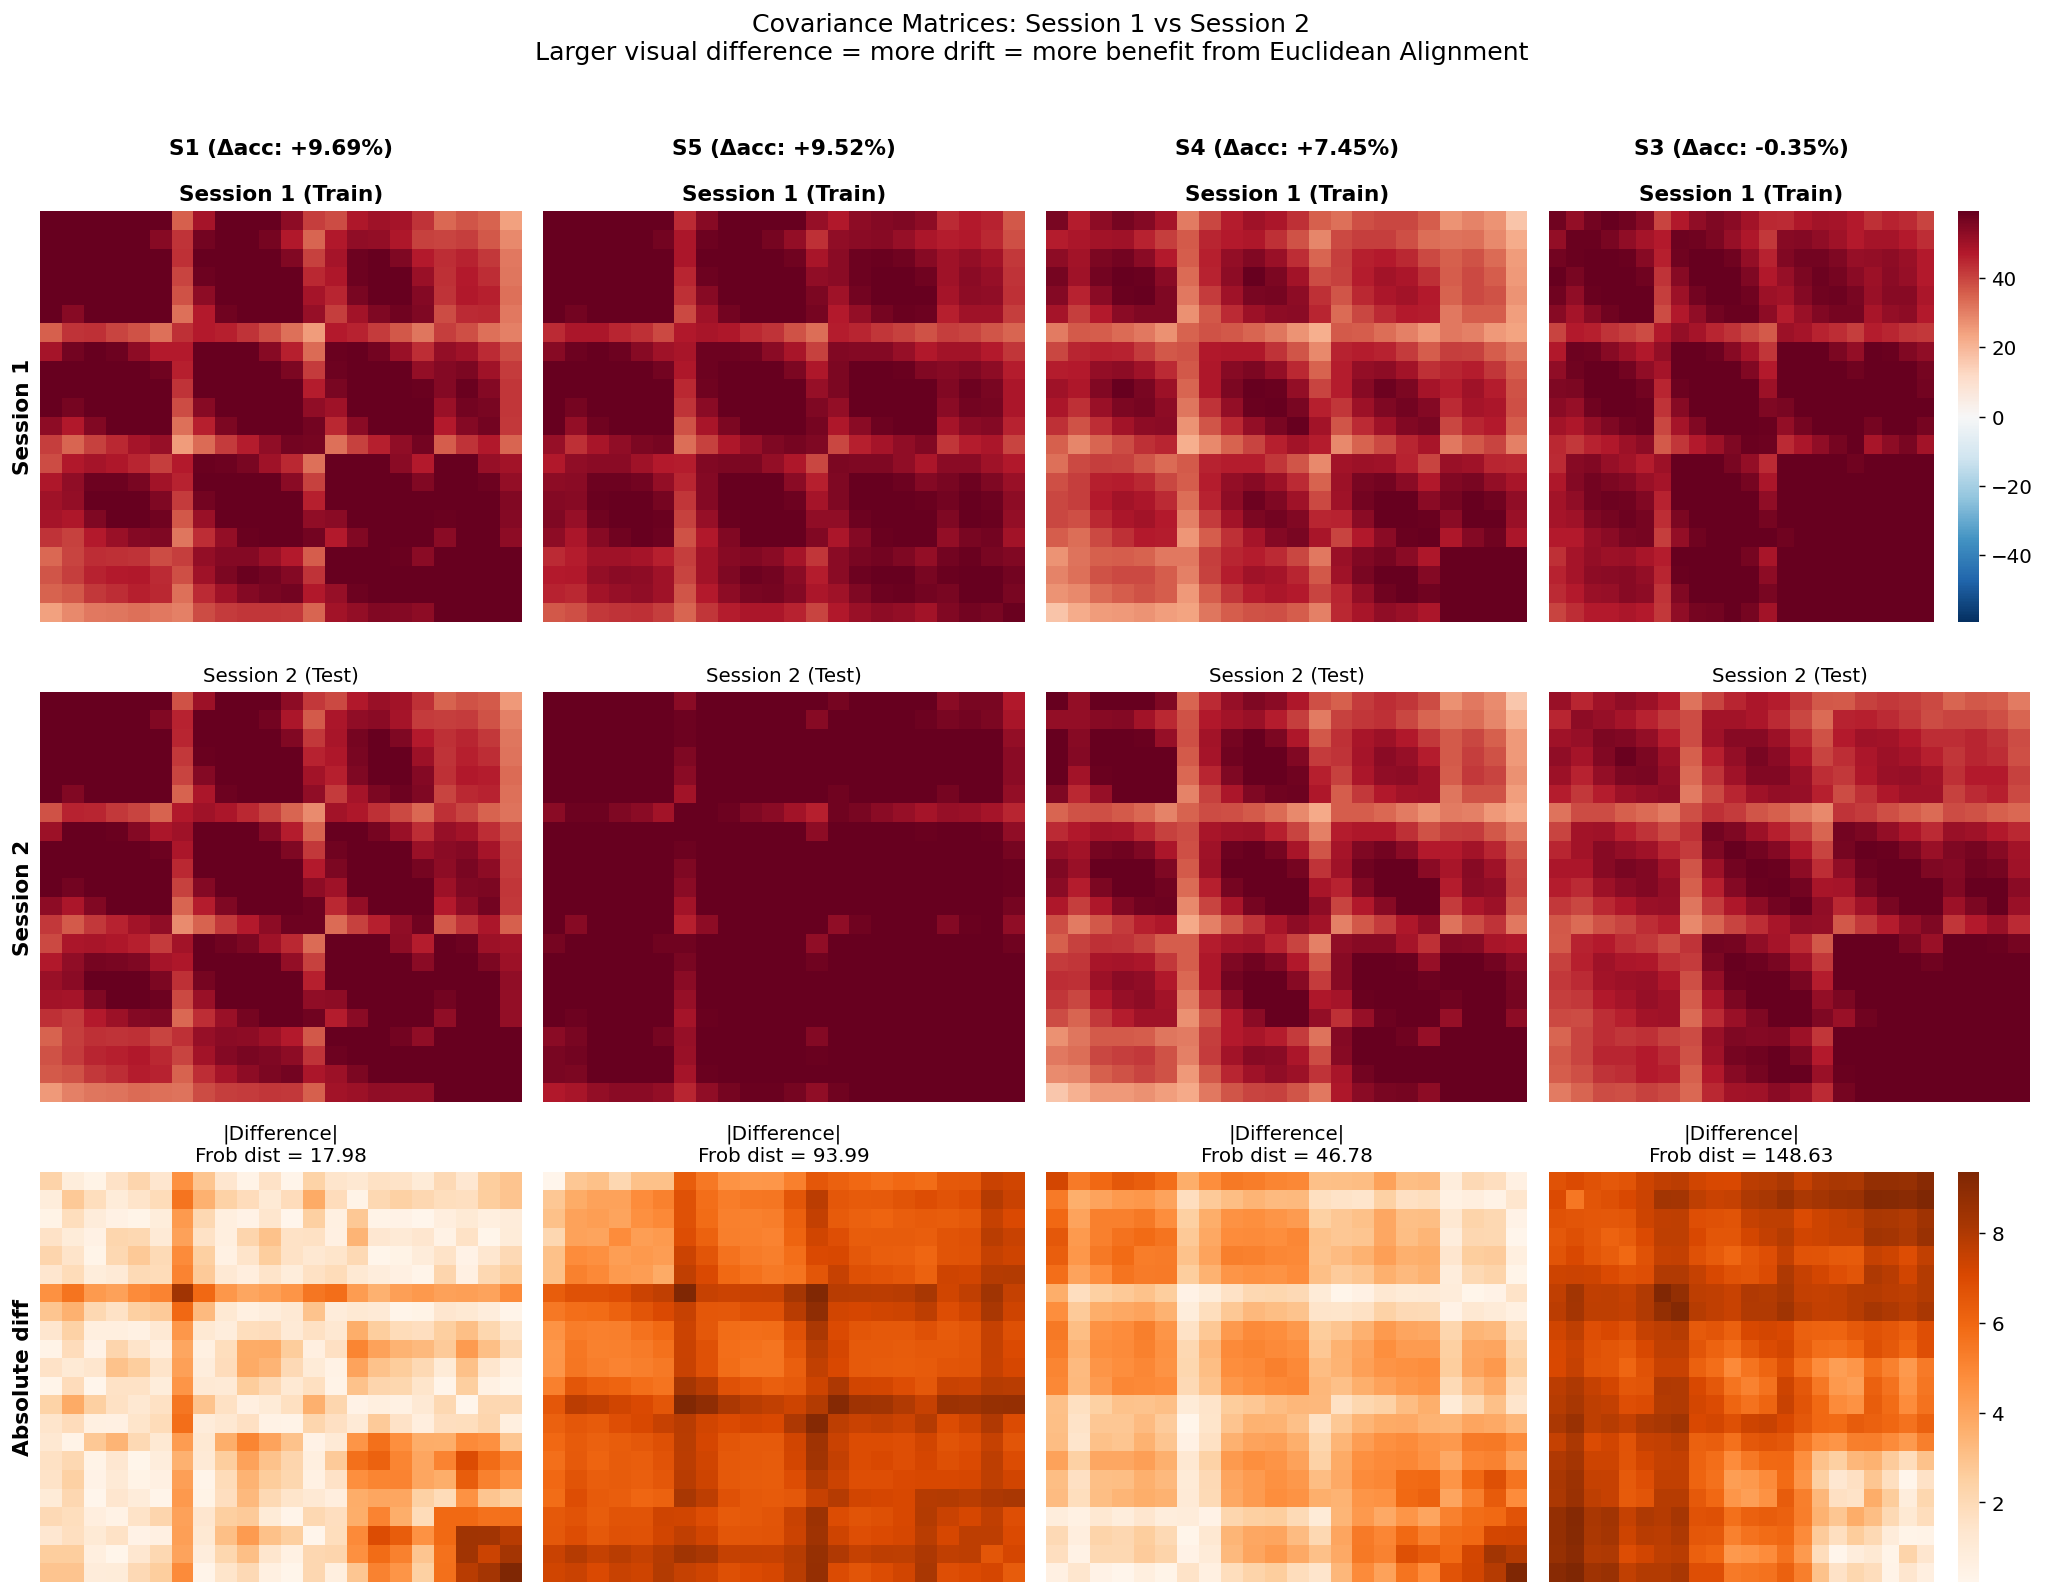
\includegraphics[width=0.9\textwidth]{fig2.png}}
\caption{Covariance heatmaps: Session 1 vs Session 2 for representative BCIC-IV-2a subjects. Larger visual difference indicates greater cross-session drift.}
\label{fig:bcic_heatmaps}
\end{figure*}

Table~\ref{tab:bcic_drift_mechanic} presents the complete per-subject covariance drift, Mu Fisher ratio, accuracy, and identified primary gain driver for each subject. Subject~2 exhibits the most extreme drift (Frobenius = 1128.21) and benefits primarily from EA. Subjects~8 and 9 follow the same pattern with large drift values. Subjects with low-to-moderate drift (S1, S4, S5, S6, S7), whose covariance manifolds are already closer across sessions, benefit primarily from the fortified ensemble pipeline---label smoothing and soft voting---confirming that these components provide substantial complementary gains when EA's marginal impact diminishes.

\begin{table*}[t]
\caption{BCIC-IV-2a --- Covariance Drift, Fisher Ratio, and Primary Driver}
\begin{center}
\begin{tabular}{|c|c|c|c|c|l|}
\hline
\textbf{Subj.} & \textbf{Cov Drift} & \textbf{Mu Fisher} & \textbf{SWCNet (\%)} & \textbf{MB-SWCNet (\%)} & \textbf{Primary Driver} \\
\hline
S1 & 17.98   & 24.16 & 78.16 & 86.81 & Multi-Band (High Fisher) \\
S2 & 1128.21 & 10.54 & 50.44 & 54.17 & EA \\
S3 & 148.63  & 43.11 & 86.81 & 89.93 & EA \\
S4 & 46.78   & 2.70  & 65.81 & 71.18 & Ensemble / Smoothing \\
S5 & 93.99   & 0.98  & 53.33 & 58.68 & Ensemble / Smoothing \\
S6 & 28.15   & 6.63  & 54.96 & 56.60 & Ensemble / Smoothing \\
S7 & 102.28  & 4.66  & 81.75 & 83.68 & Ensemble / Smoothing \\
S8 & 245.38  & 15.60 & 79.17 & 83.33 & EA \\
S9 & 122.80  & 35.22 & 75.83 & 81.60 & EA + Multi-Band \\
\hline
\end{tabular}
\label{tab:bcic_drift_mechanic}
\end{center}
\end{table*}

\begin{figure*}[t]
\centerline{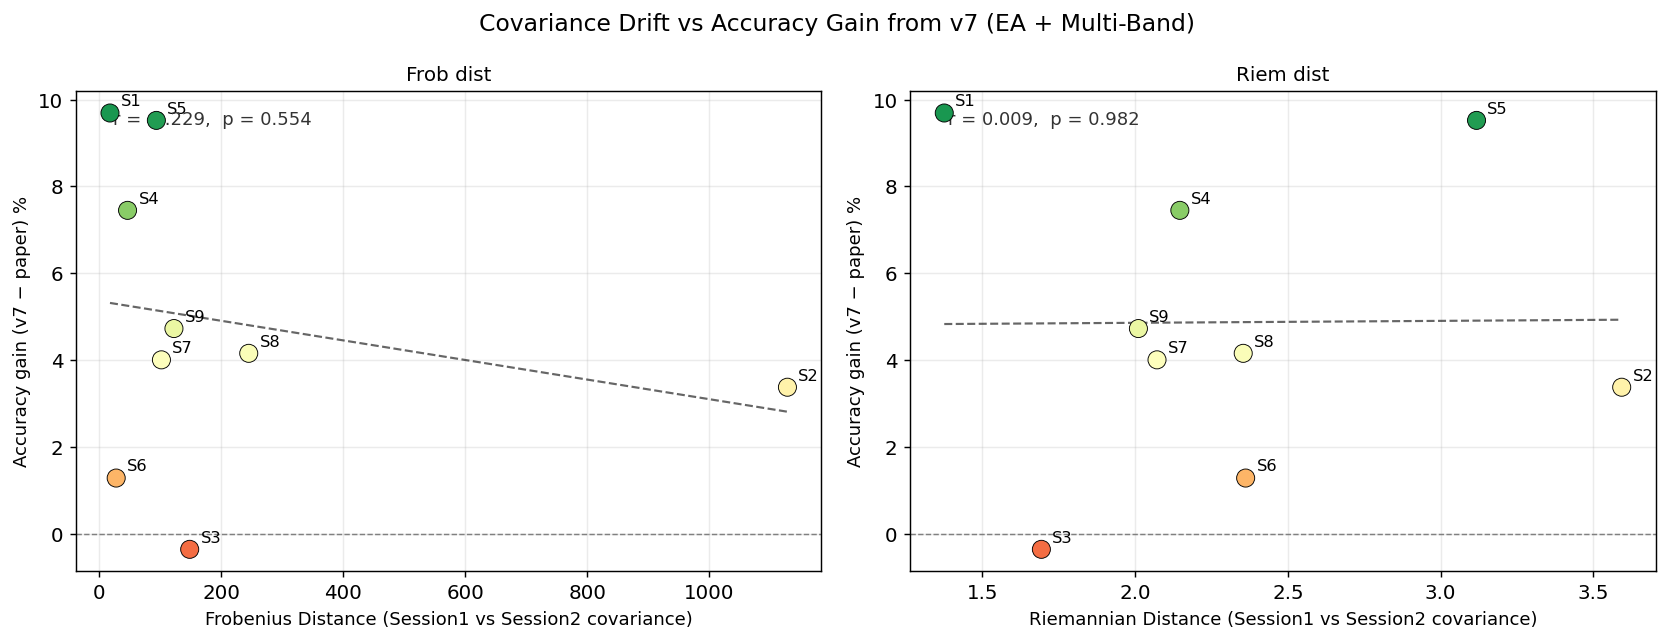
\includegraphics[width=0.75\textwidth]{fig3.png}}
\caption{Scatter: Covariance drift (Frobenius distance) vs.\ accuracy gain per subject on BCIC-IV-2a.}
\label{fig:bcic_scatter}
\end{figure*}

\subsubsection*{Spectral Discriminability Across Frequency Bands}

To quantitatively justify the multi-band decomposition on BCIC-IV-2a, we compute the Fisher ratio (between-class variance divided by within-class variance) for each frequency band, aggregated across all 9 subjects. The results are presented in Table~\ref{tab:bcic_fisher} alongside the PSD comparison at motor electrodes in Fig.~\ref{fig:bcic_psd}.

\begin{figure*}[t]
\centerline{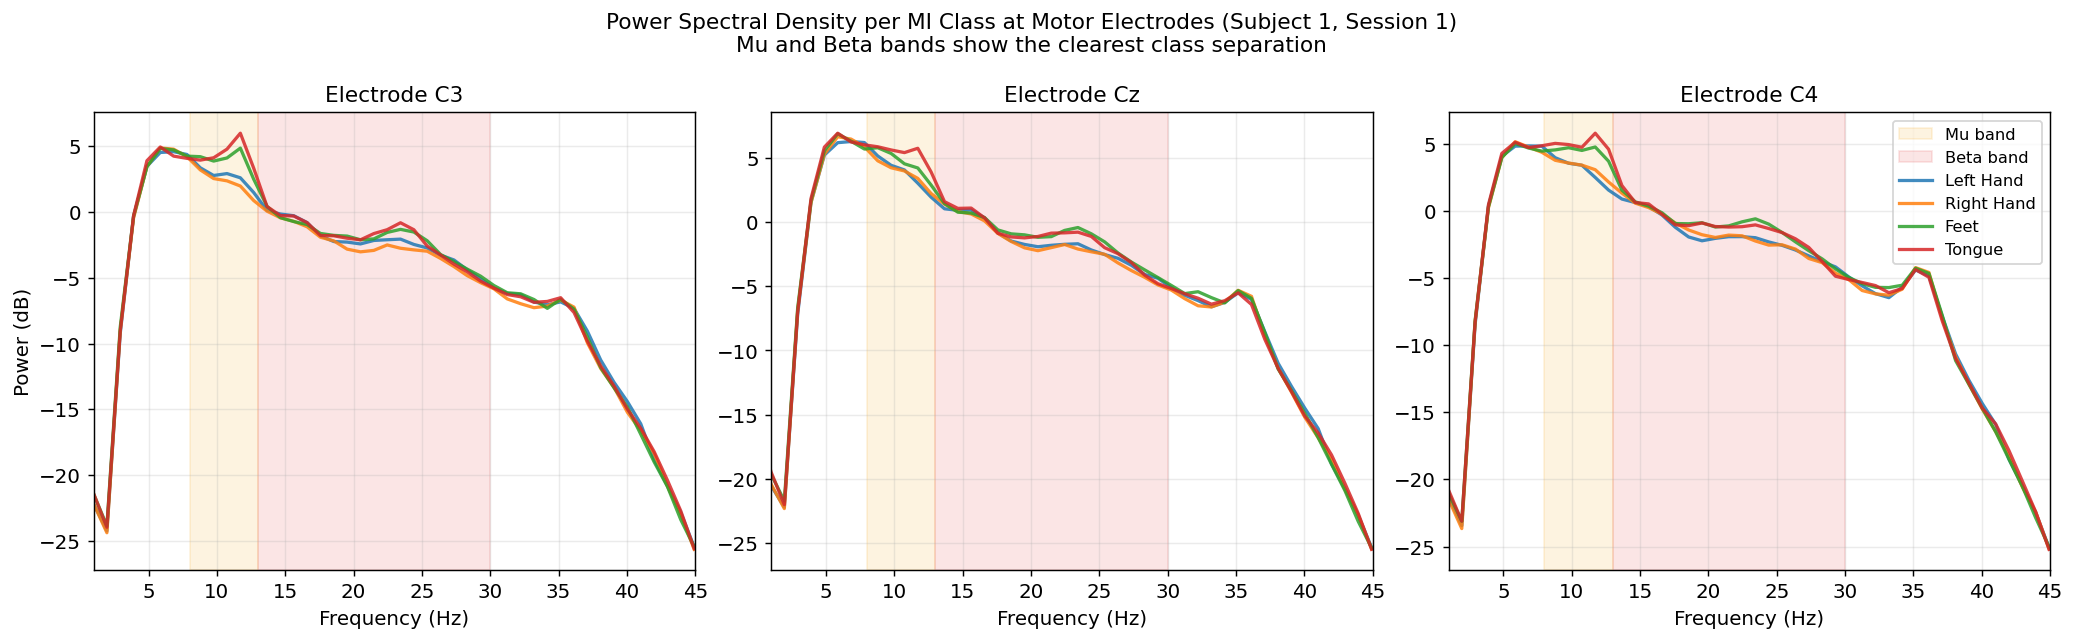
\includegraphics[width=0.85\textwidth]{fig4.png}}
\caption{PSD per MI class at C3, Cz, C4 (Subject 1, Session 1).}
\label{fig:bcic_psd}
\end{figure*}

The Mu band emerges as the most class-discriminative frequency range, with a Fisher ratio of 15.17---31\% higher than broadband (11.57) and nearly $3\times$ higher than Beta (5.16). This quantitative gap directly justifies the inclusion of targeted band decomposition: a broadband classifier is inherently exposed to frequency ranges that contribute noise relative to signal, whereas the $(3C,1)$ spatial kernel can learn to weight the Mu-dominant channels when given explicit access to band-separated representations.

\begin{table}[h]
\caption{Fisher Ratio per Frequency Band --- BCIC-IV-2a}
\begin{center}
\begin{tabular}{|l|c|c|}
\hline
\textbf{Band} & \textbf{Frequency Range} & \textbf{Fisher Ratio} \\
\hline
Mu        & 8--13 Hz  & \textbf{15.17} \\
Broadband & 4--40 Hz  & 11.57 \\
Beta      & 13--30 Hz & 5.16 \\
Theta     & 4--8 Hz   & 3.16 \\
Delta     & 1--4 Hz   & 1.76 \\
Gamma     & 30--40 Hz & 1.38 \\
\hline
\end{tabular}
\label{tab:bcic_fisher}
\end{center}
\end{table}

\subsection{High Gamma Dataset: Geometric Alignment and Subject Heterogeneity}

\subsubsection*{Geometric Effect of Euclidean Alignment}

To evaluate how EA reshapes the distribution of cross-session features on HGD, we compute t-SNE embeddings of spatial covariance features for representative subjects before and after alignment. Figures~\ref{fig:hgd_tsne_ab} and~\ref{fig:hgd_tsne_cd} present the results for four subjects spanning the observed gain range.

\begin{figure*}[t]
\centering
  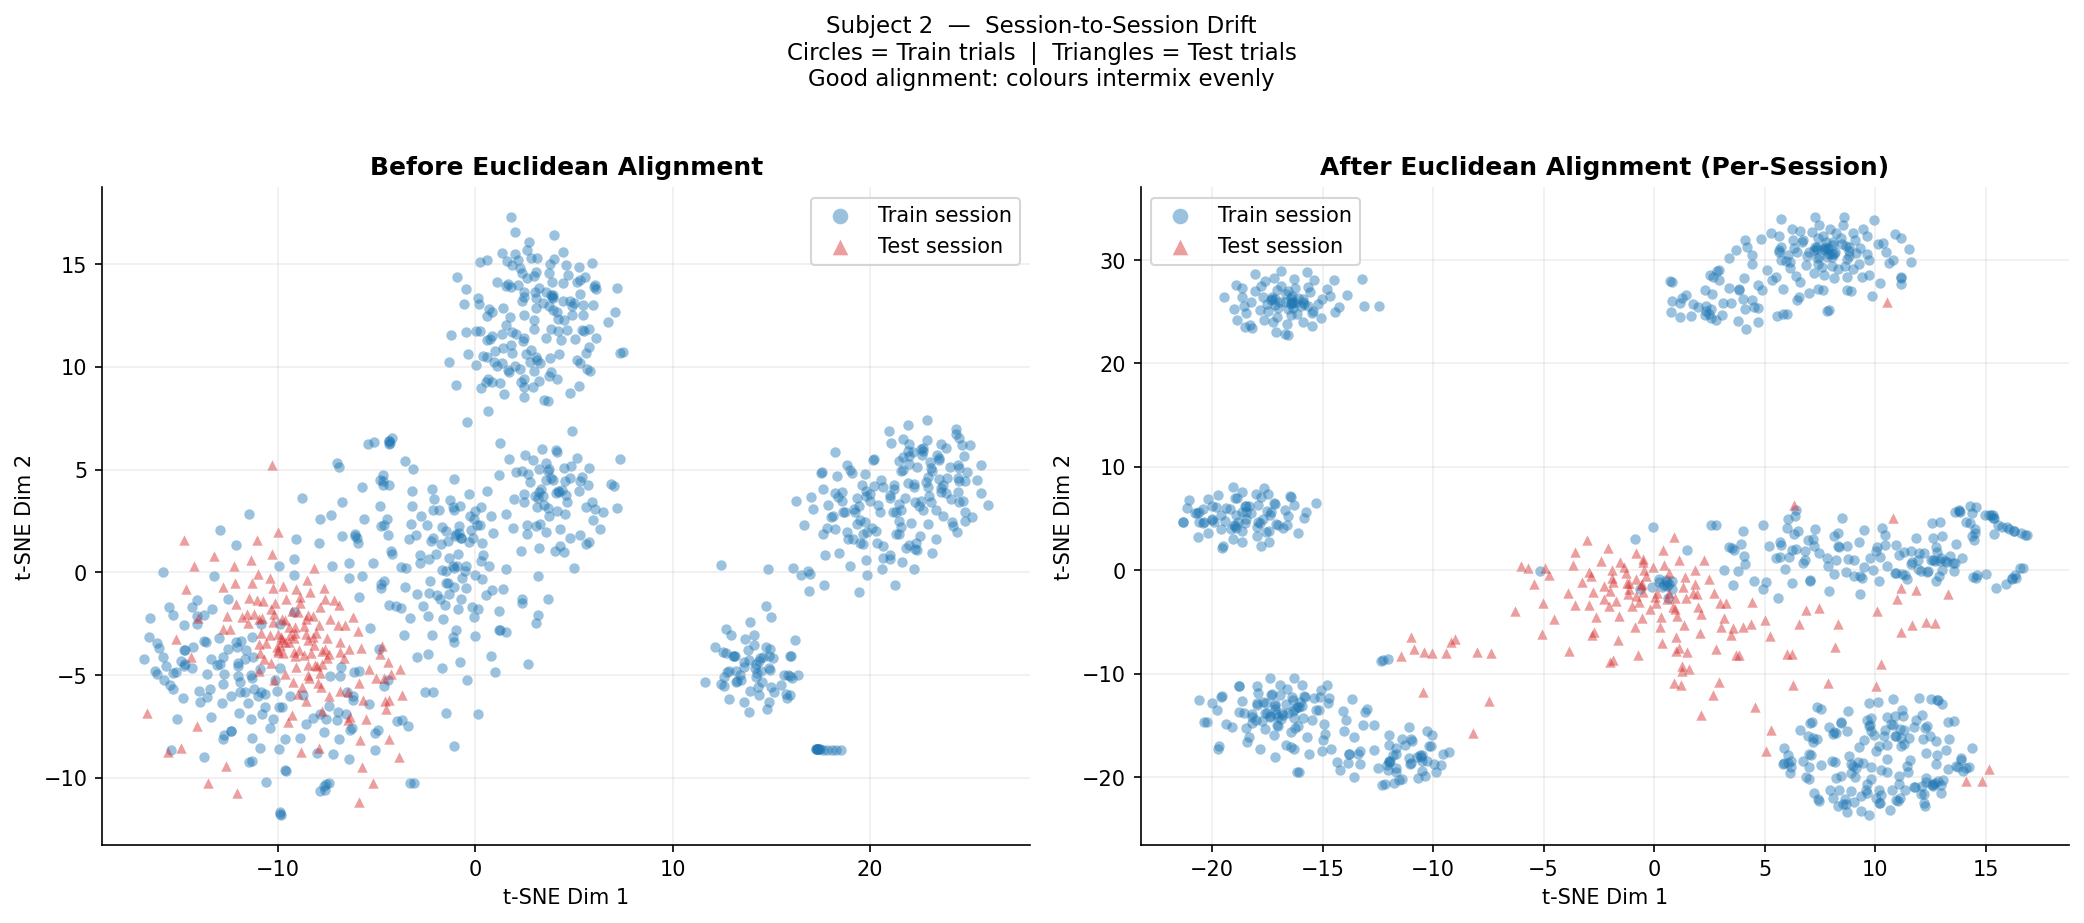
\includegraphics[width=0.8\textwidth]{exp1_tsne_session_drift_s2.png}\\[0.4em]
  \small (a) Subject 2\\[0.8em]
  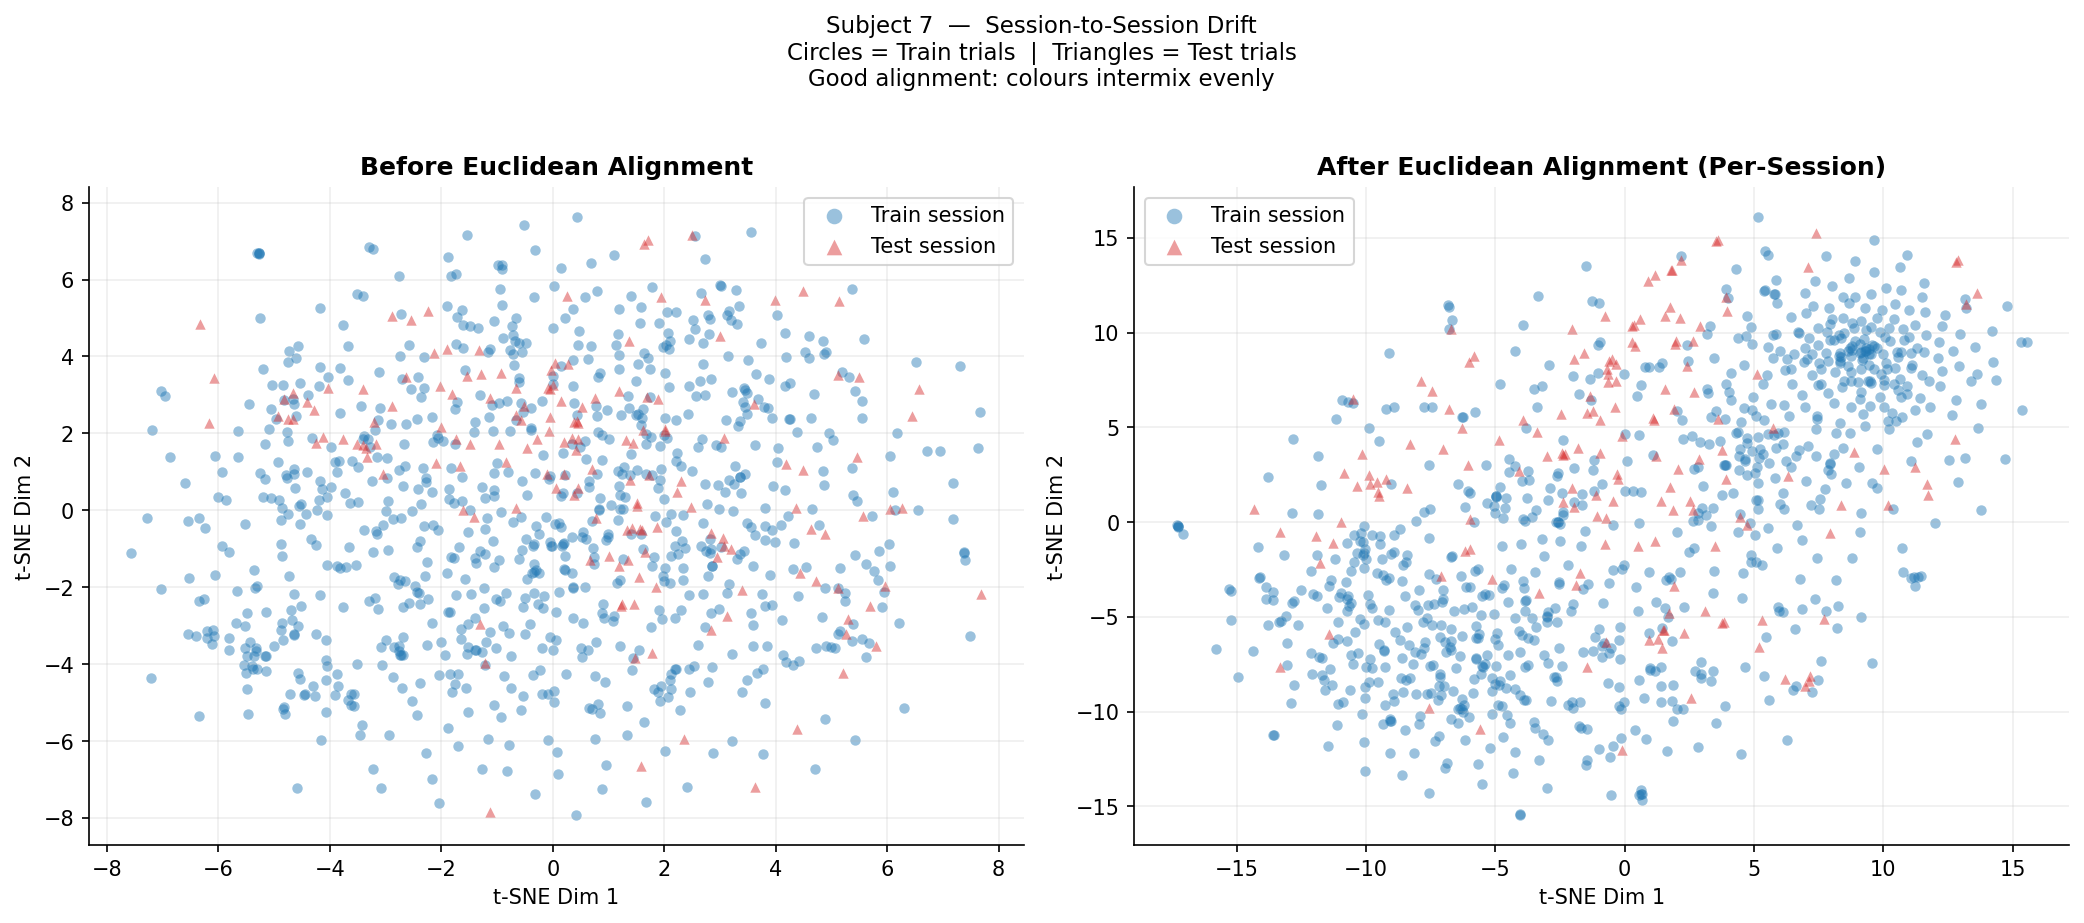
\includegraphics[width=0.8\textwidth]{exp1_tsne_session_drift_s7.png}\\[0.4em]
  \small (b) Subject 7
\caption{t-SNE visualization of HGD deep latent features before and after Euclidean Alignment (Subjects 2 and 7): successful neutralization of inter-session distributional shift.}
\label{fig:hgd_tsne_ab}
\end{figure*}

\begin{figure*}[t]
\centering
  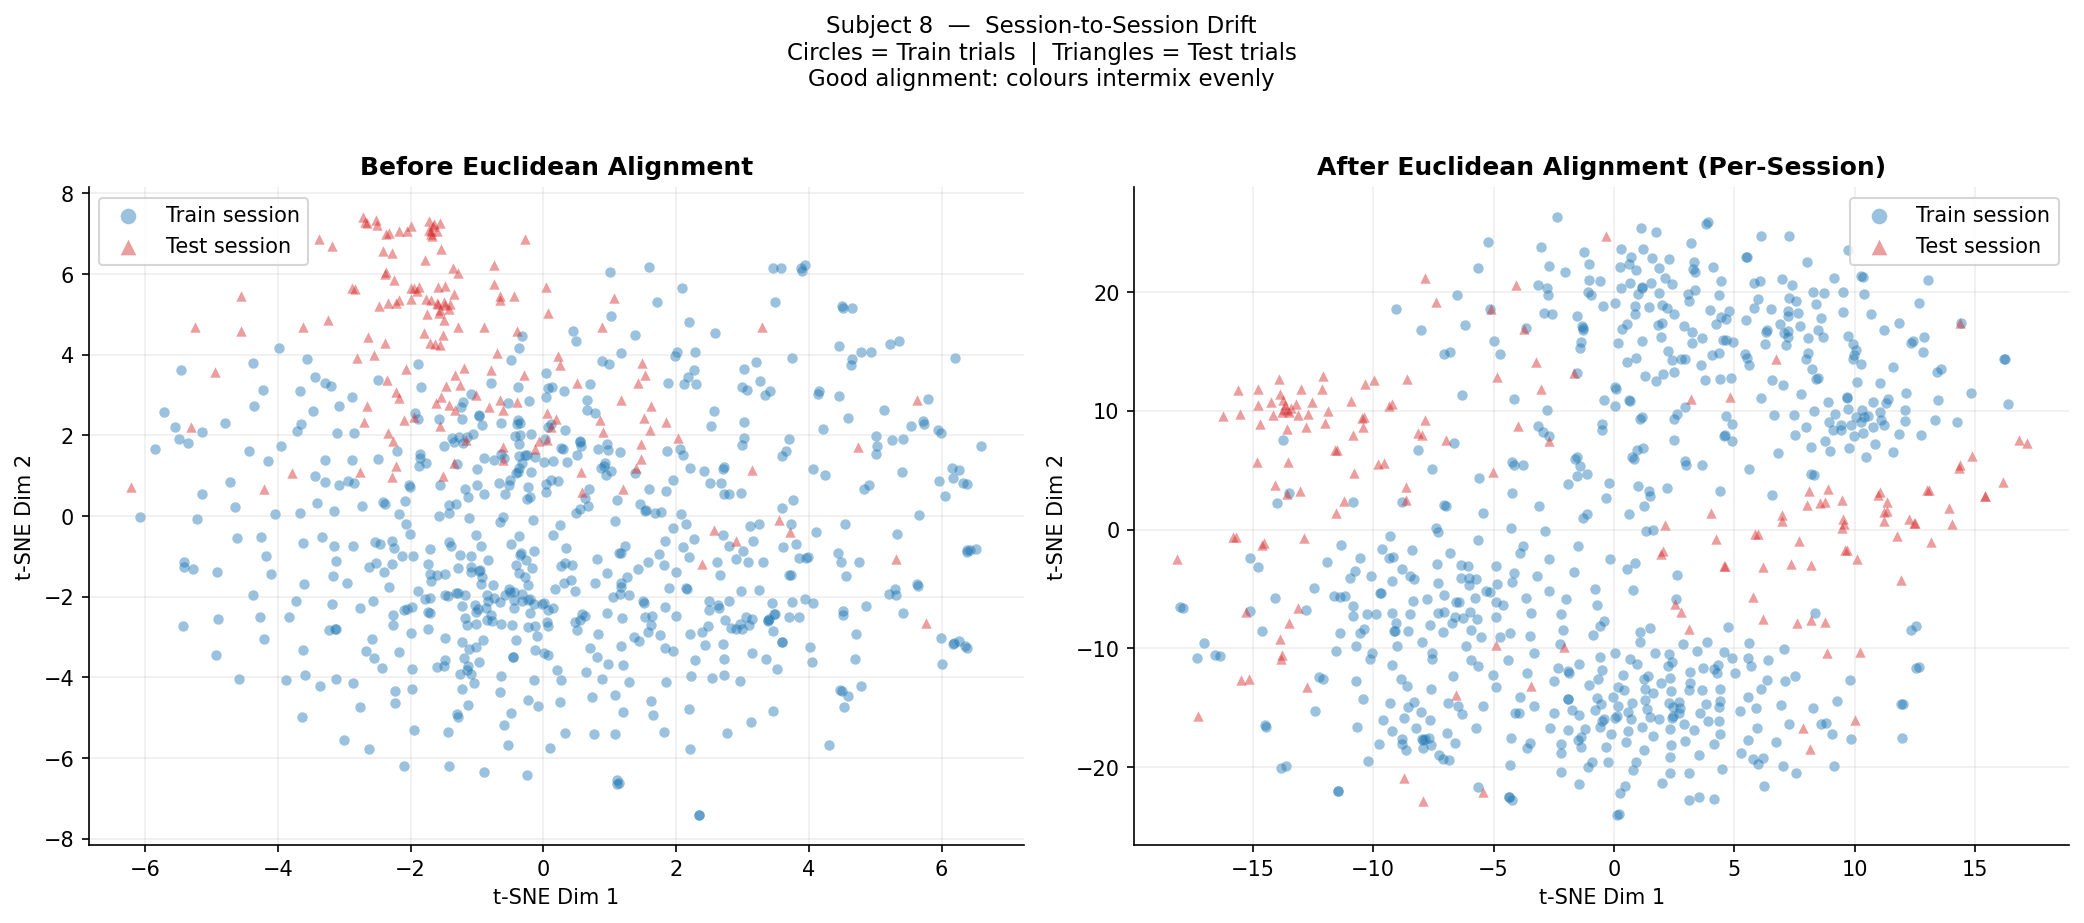
\includegraphics[width=0.8\textwidth]{exp1_tsne_session_drift_s8.png}\\[0.4em]
  \small (c) Subject 8\\[0.8em]
  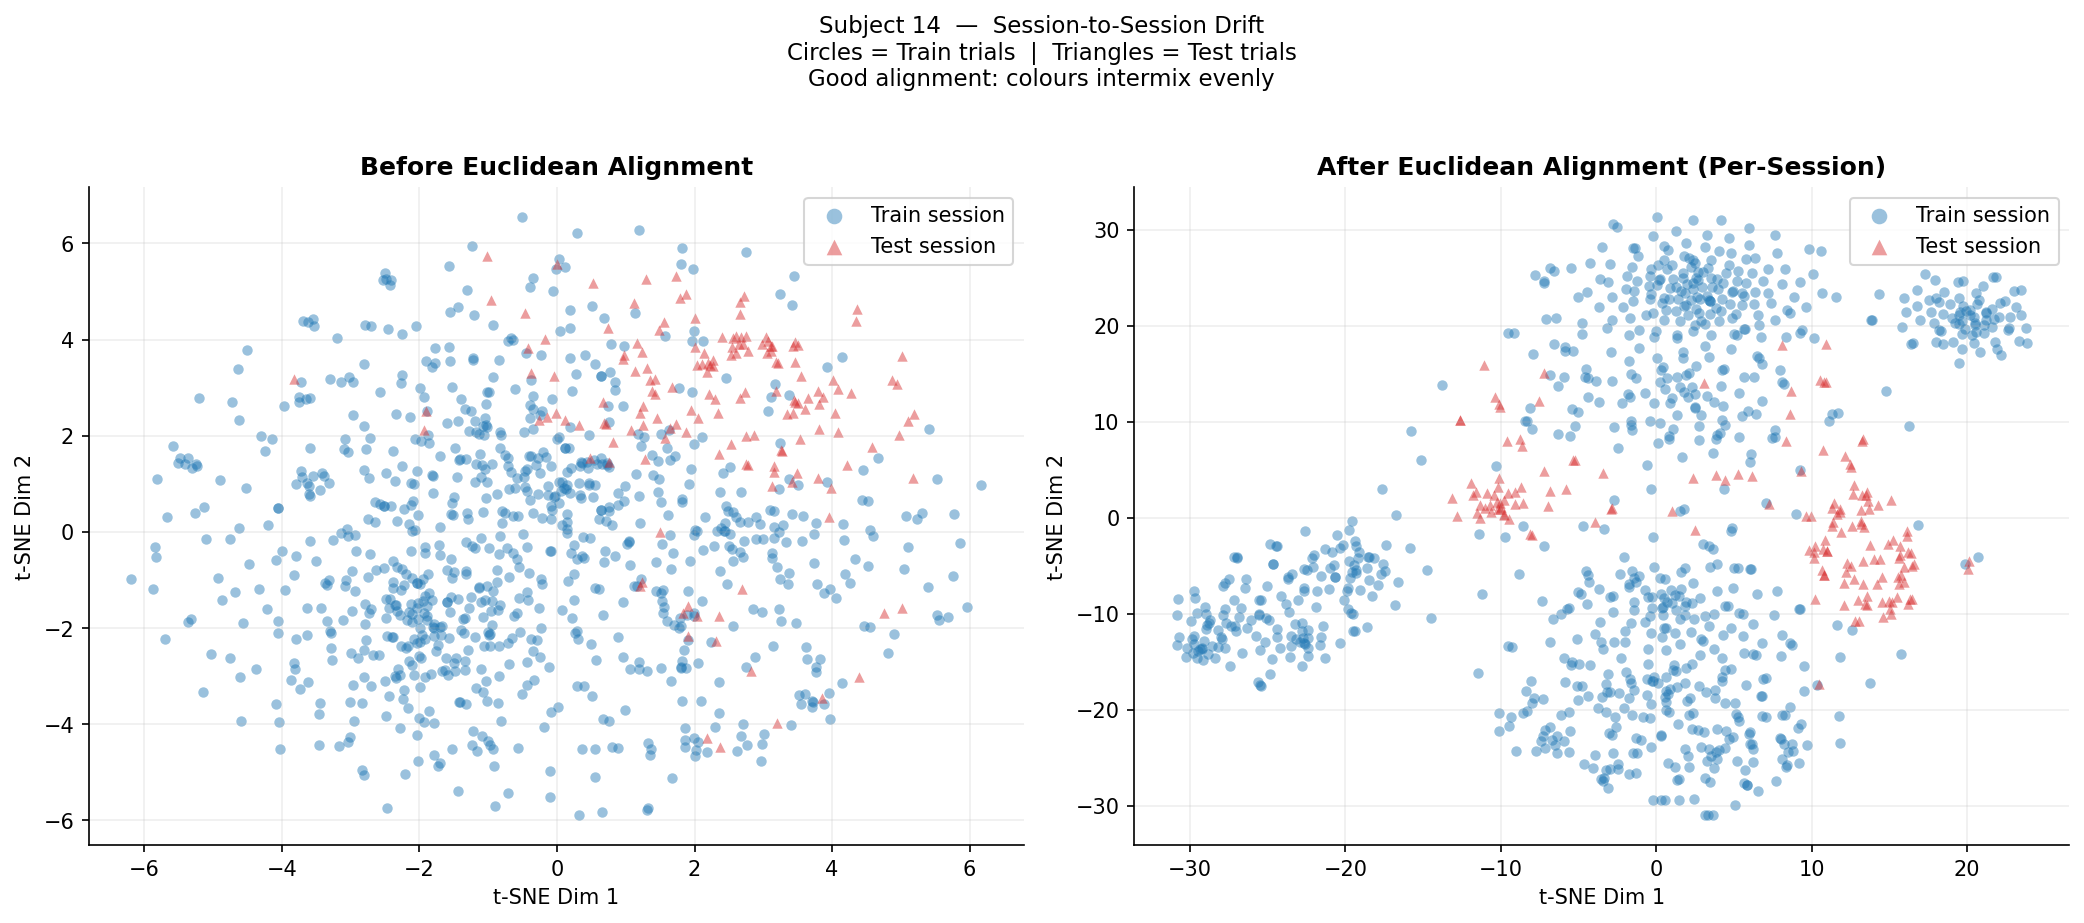
\includegraphics[width=0.8\textwidth]{exp1_tsne_session_drift_s14.png}\\[0.4em]
  \small (d) Subject 14
\caption{t-SNE visualization of HGD deep latent features before and after Euclidean Alignment (Subjects 8 and 14): continued.}
\label{fig:hgd_tsne_cd}
\end{figure*}

For subjects with high inter-session drift---such as S2, S8, and S14---the pre-alignment embeddings show clearly separated train and test clusters, which collapse into a well-intermixed joint distribution after EA. For S7, where the native drift was smaller but still measurable, alignment similarly reduces cluster separation and produces the large +15\% accuracy gain shown in Table~\ref{tab:hgd_combined}.

\subsubsection*{Stable-Manifold Subjects: When Alignment Hurts}

We introduce the formal term \textbf{Stable-Manifold Subjects} to replace the descriptive label ``Decrease Subjects'' with one that reflects the underlying physiological reality. A Stable-Manifold Subject is one whose inter-session EEG covariance shift is below the threshold at which EA provides net benefit, typically characterised by both high native cross-session accuracy and attenuated canonical ERD peaks.

Figure~\ref{fig:hgd_psd_surge} presents power spectral density profiles for three HGD subjects: S3 (a high performer with strong Mu/Beta power), alongside S5 and S9 who are representative Stable-Manifold Subjects. The PSD of S5 and S9 shows substantially attenuated Mu and Beta peaks relative to S3, confirming that their MI-related spectral signatures are weaker---meaning expanded frequency channels supply noise rather than additional discriminative signal.

\begin{figure*}[!t]
  \setlength{\abovecaptionskip}{4pt}
  \centering
  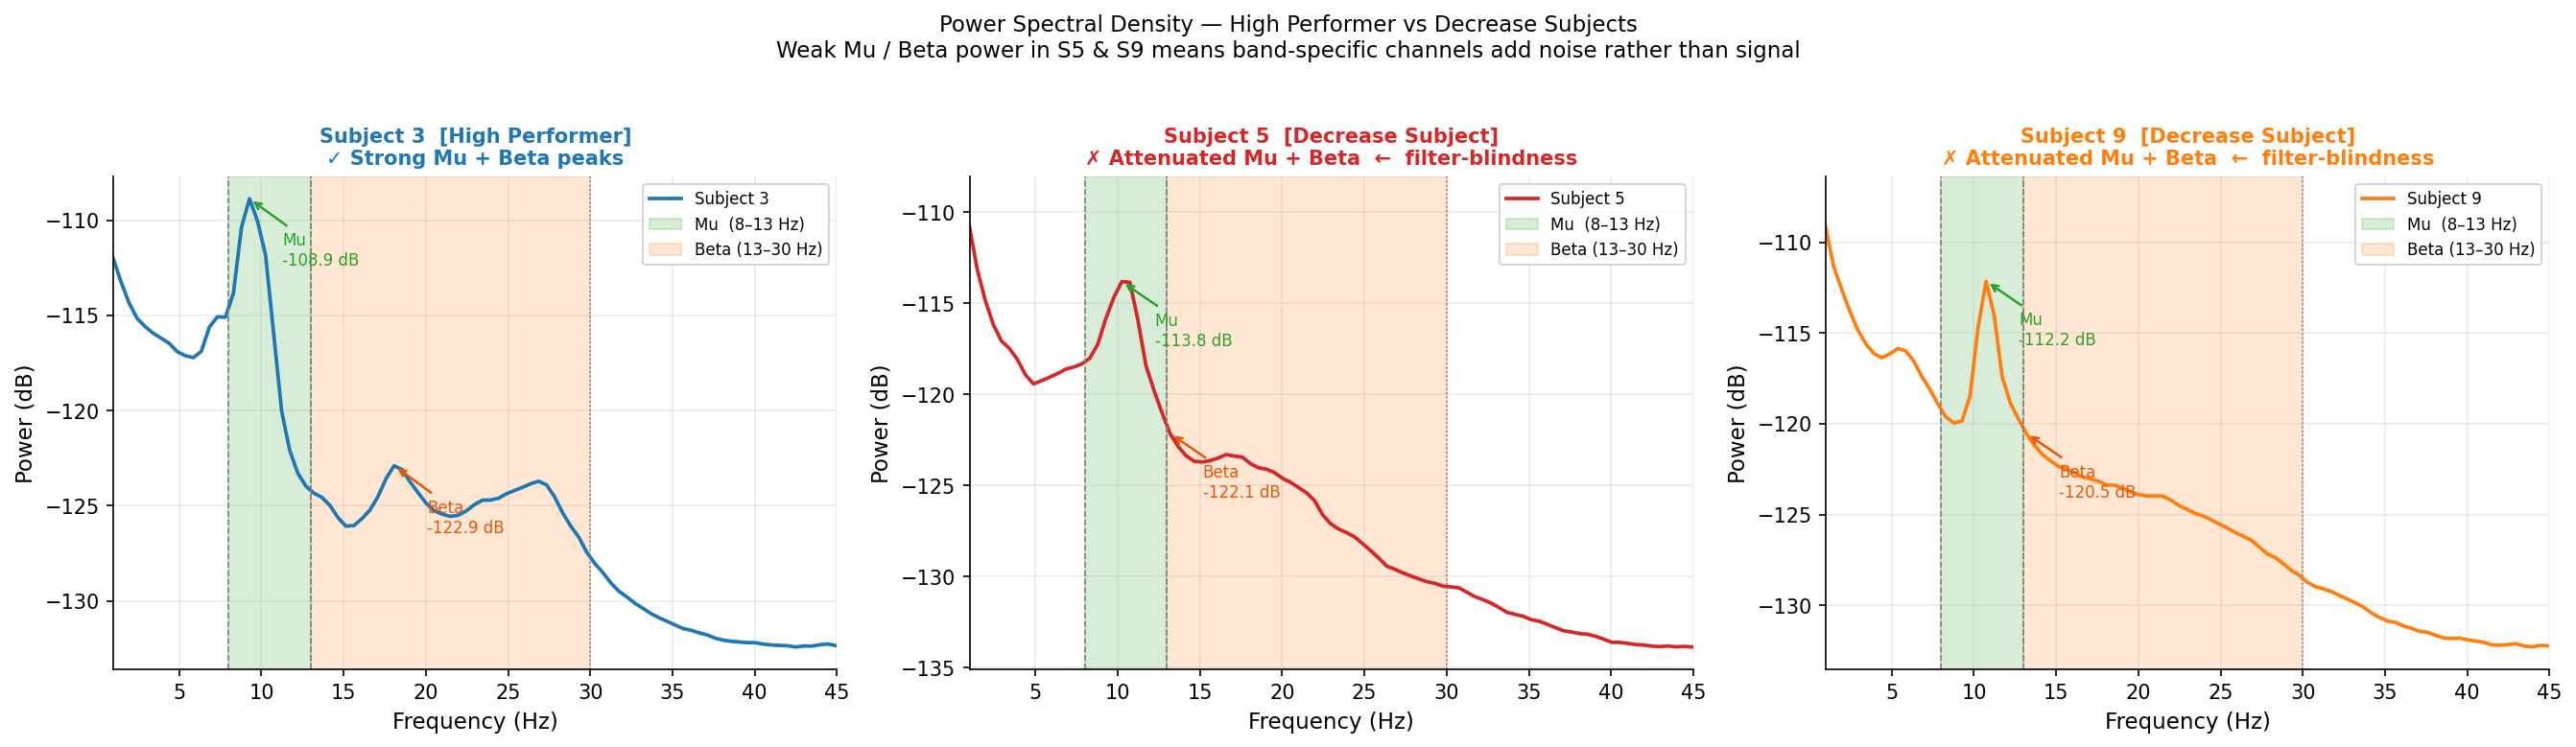
\includegraphics[width=0.92\textwidth]{exp2_psd_s3_s5_s9.png}
  \caption{Three-panel PSD: S3 (High Performer) $|$ S5 (Stable-Manifold)
           $|$ S9 (Stable-Manifold).}
  \label{fig:hgd_psd_surge}
\end{figure*}

\subsubsection*{Component Ablation on HGD}

To isolate the contribution of each proposed novelty, we conducted a controlled per-component ablation study on S5 (Stable-Manifold Subject, $-20.91$\%) and S14 (Surge Subject, $+26.50$\%) across four conditions. Results are presented in Table~\ref{tab:ablation_mechanic} and Fig.~\ref{fig:hgd_ablation}.

\begin{table*}[!t]
\caption{Ablation Study --- HGD Setup II (S5: Stable-Manifold Subject, S14: Surge Subject)}
\begin{center}
\setlength{\tabcolsep}{4pt}
\begin{tabular}{|l|c|c|c||c|c||c|c|}
\hline
\textbf{Condition} & \textbf{EA} & \textbf{Bands} & \textbf{Chans.} &
\textbf{S5 CV} & \textbf{S5 Test} &
\textbf{S14 CV} & \textbf{S14 Test} \\
\hline
Baseline  & \ding{55} & 1 & 44  & 97.64\% & 97.50\% & 98.98\% & 96.25\% \\
EA Only   & \ding{51} & 1 & 44  & 96.81\% & 67.50\% & 99.20\% & 95.62\% \\
MB Only   & \ding{55} & 3 & 132 & 95.97\% & 97.50\% & 98.75\% & 96.88\% \\
Proposed  & \ding{51} & 3 & 132 & 96.53\% & 79.38\% & 98.86\% & 95.62\% \\
\hline
\end{tabular}
\label{tab:ablation_mechanic}
\end{center}
\end{table*}

\begin{figure*}[!t]
  \setlength{\abovecaptionskip}{4pt}
  \centering
  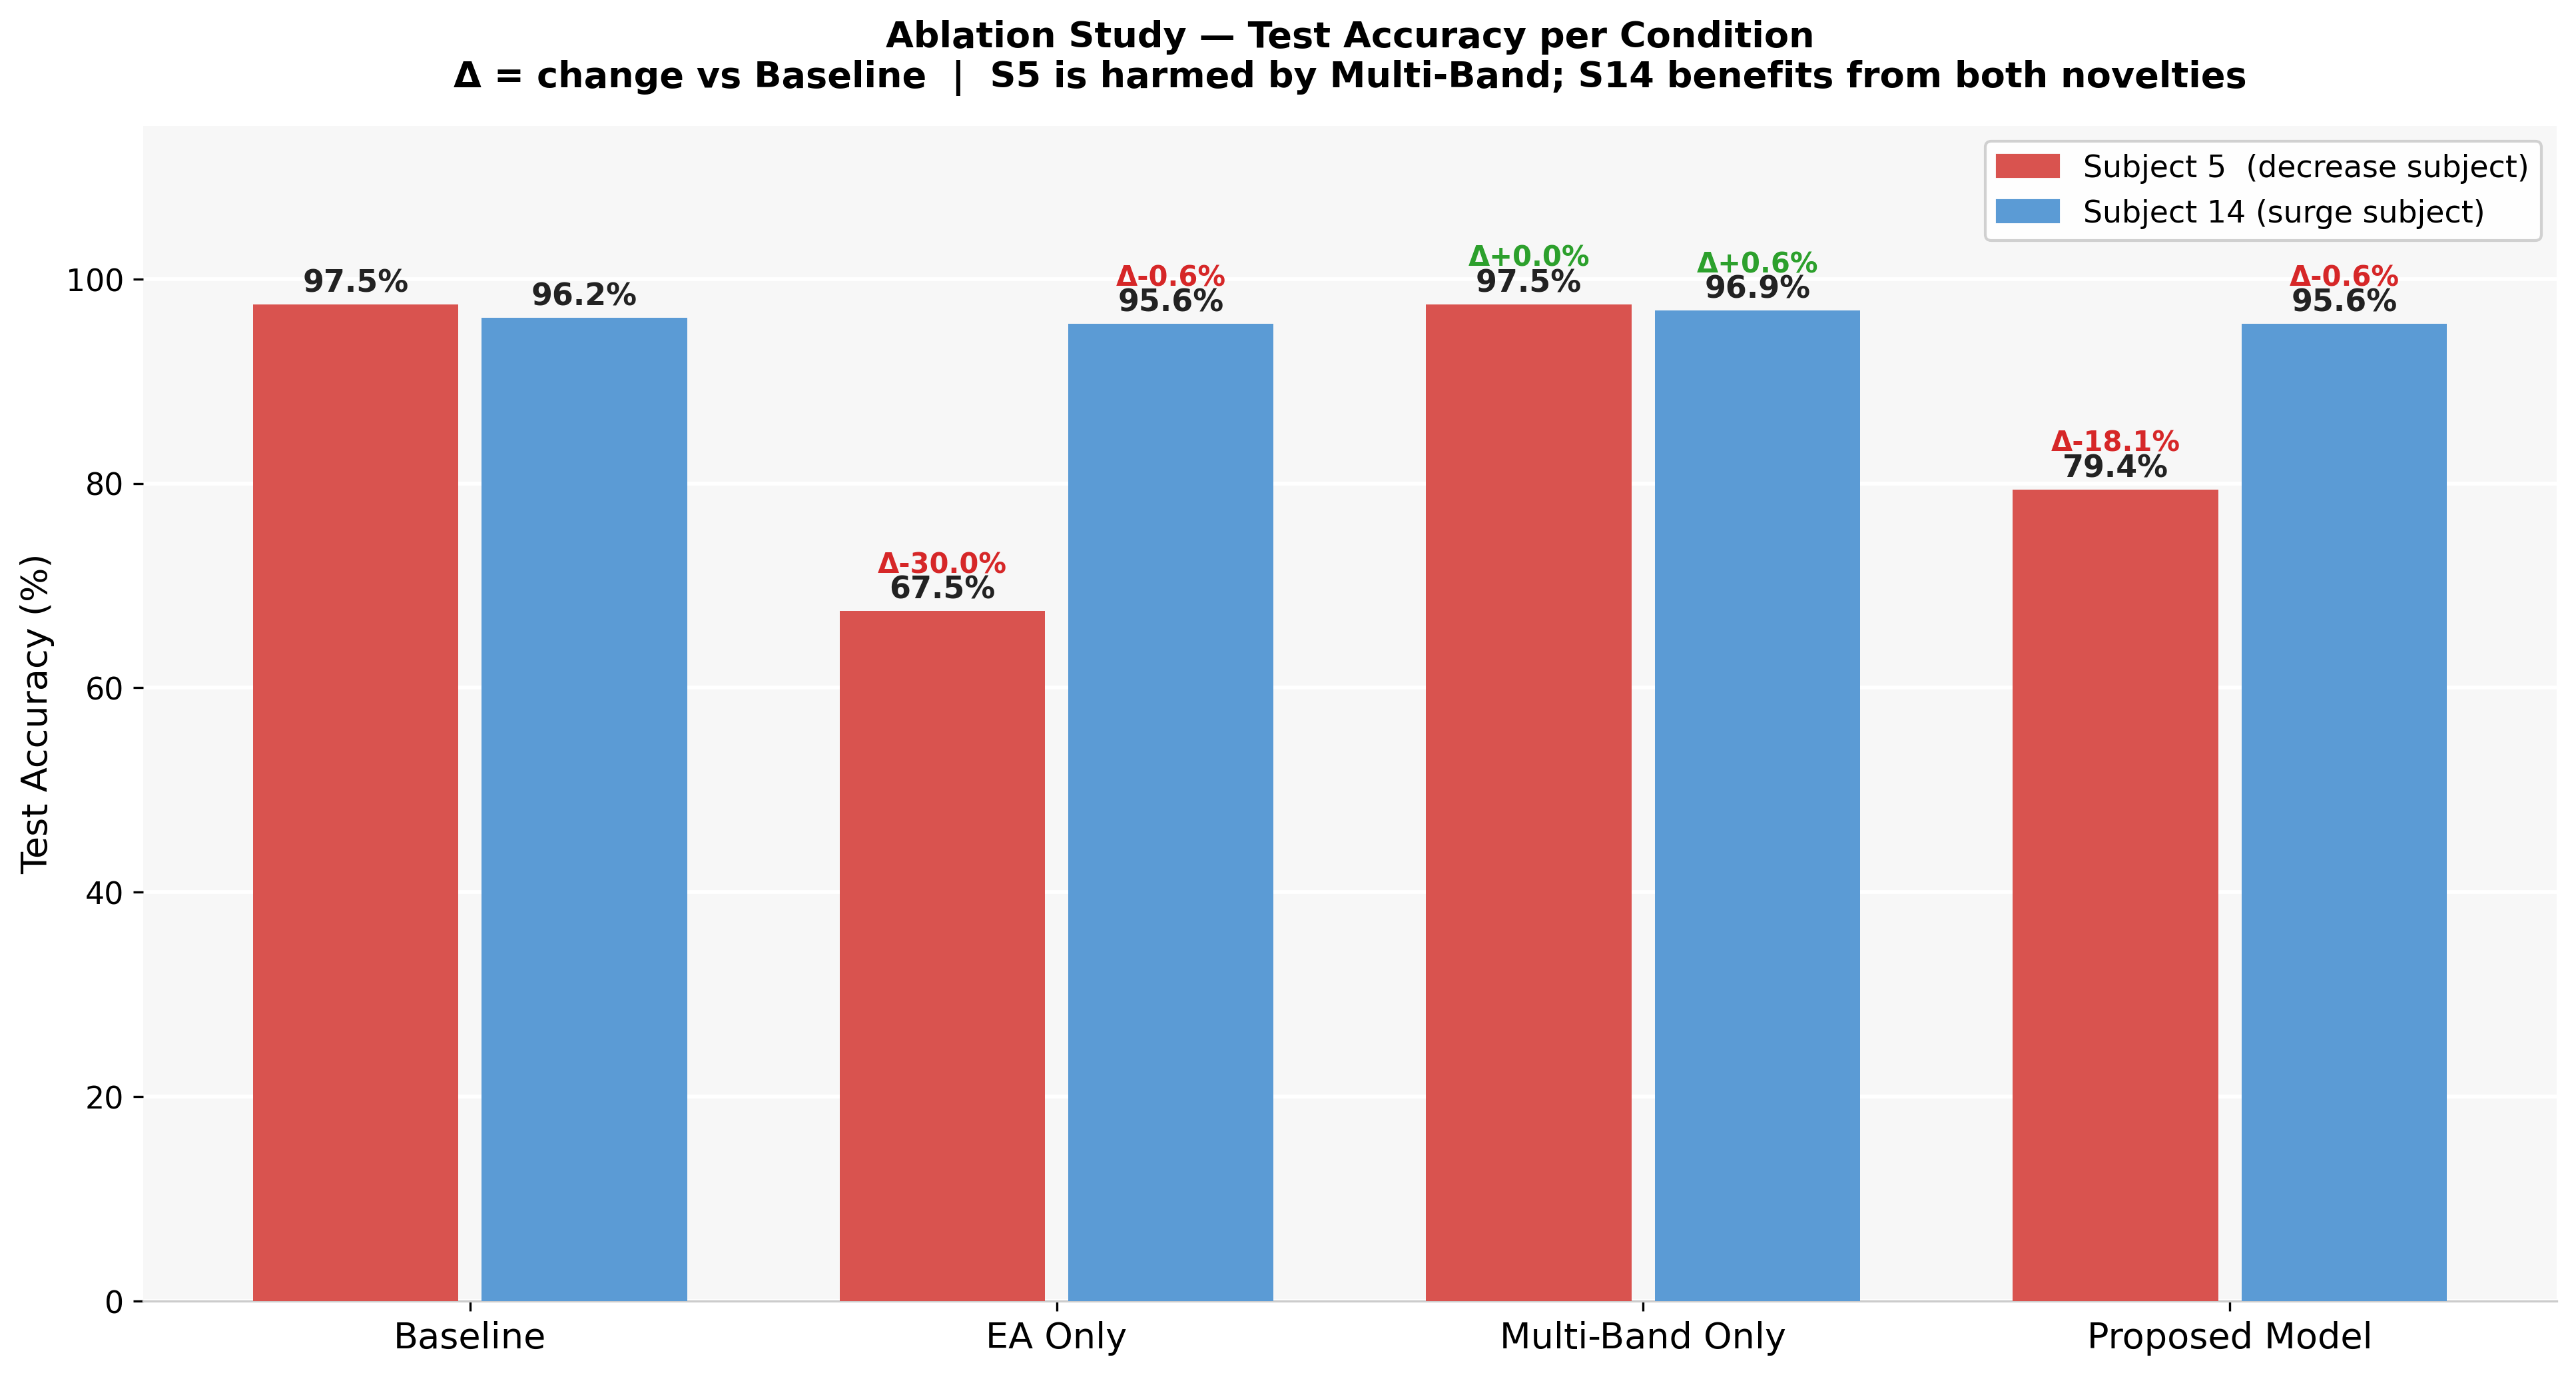
\includegraphics[width=0.82\textwidth]{exp3_ablation_s5_s14.png}
  \caption{Subject-level ablation results on HGD: S14 (Surge Subject)
           benefits from the proposed model while S5 (Stable-Manifold
           Subject) illustrates the negative transfer boundary condition.}
  \label{fig:hgd_ablation}
\end{figure*}

The ablation reveals two complementary findings. For S14, each component contributes positively: EA corrects the large inter-session covariance gap, and multi-band decomposition then amplifies class-specific spectral signatures that EA has geometrically stabilised. For S5, the picture reverses sharply. The ``EA Only'' condition drops test accuracy by 30.00\% while cross-validation accuracy on the training session remains high at 96.81\%---a pattern we term the \textbf{CV-Test Dissociation Effect}. The dissociation arises because EA distorts a spatial manifold that was already consistent across sessions: the alignment transformation introduces geometric noise rather than correcting a genuine shift, and this distortion only becomes apparent on the held-out Day~2 data where the model encounters the corrupted representation.

\subsection{OpenBMI: Population-Scale Replication}

To extend the mechanistic framework to the population-scale dataset, we conducted targeted component ablation and PSD analyses on two representative OpenBMI subjects: S2 (a Surge Subject, Setup~II accuracy = 76.00\%) and S38 (a Stable-Manifold Subject, Setup~II accuracy = 51.00\%). These subjects were selected because they exhibit contrasting response profiles while both having sufficient PSD signal quality for reliable spectral analysis. S38 mirrors the Stable-Manifold pattern identified in HGD, providing cross-dataset replication of that phenomenon at 62 channels.

\subsubsection*{Component Ablation on OpenBMI}

Fig.~\ref{fig:openbmi_ablation} presents the four-condition ablation for S2 and S38 against their respective SWCNet paper baselines (72.5\% and 58.1\%).

\begin{figure}[t]
\centerline{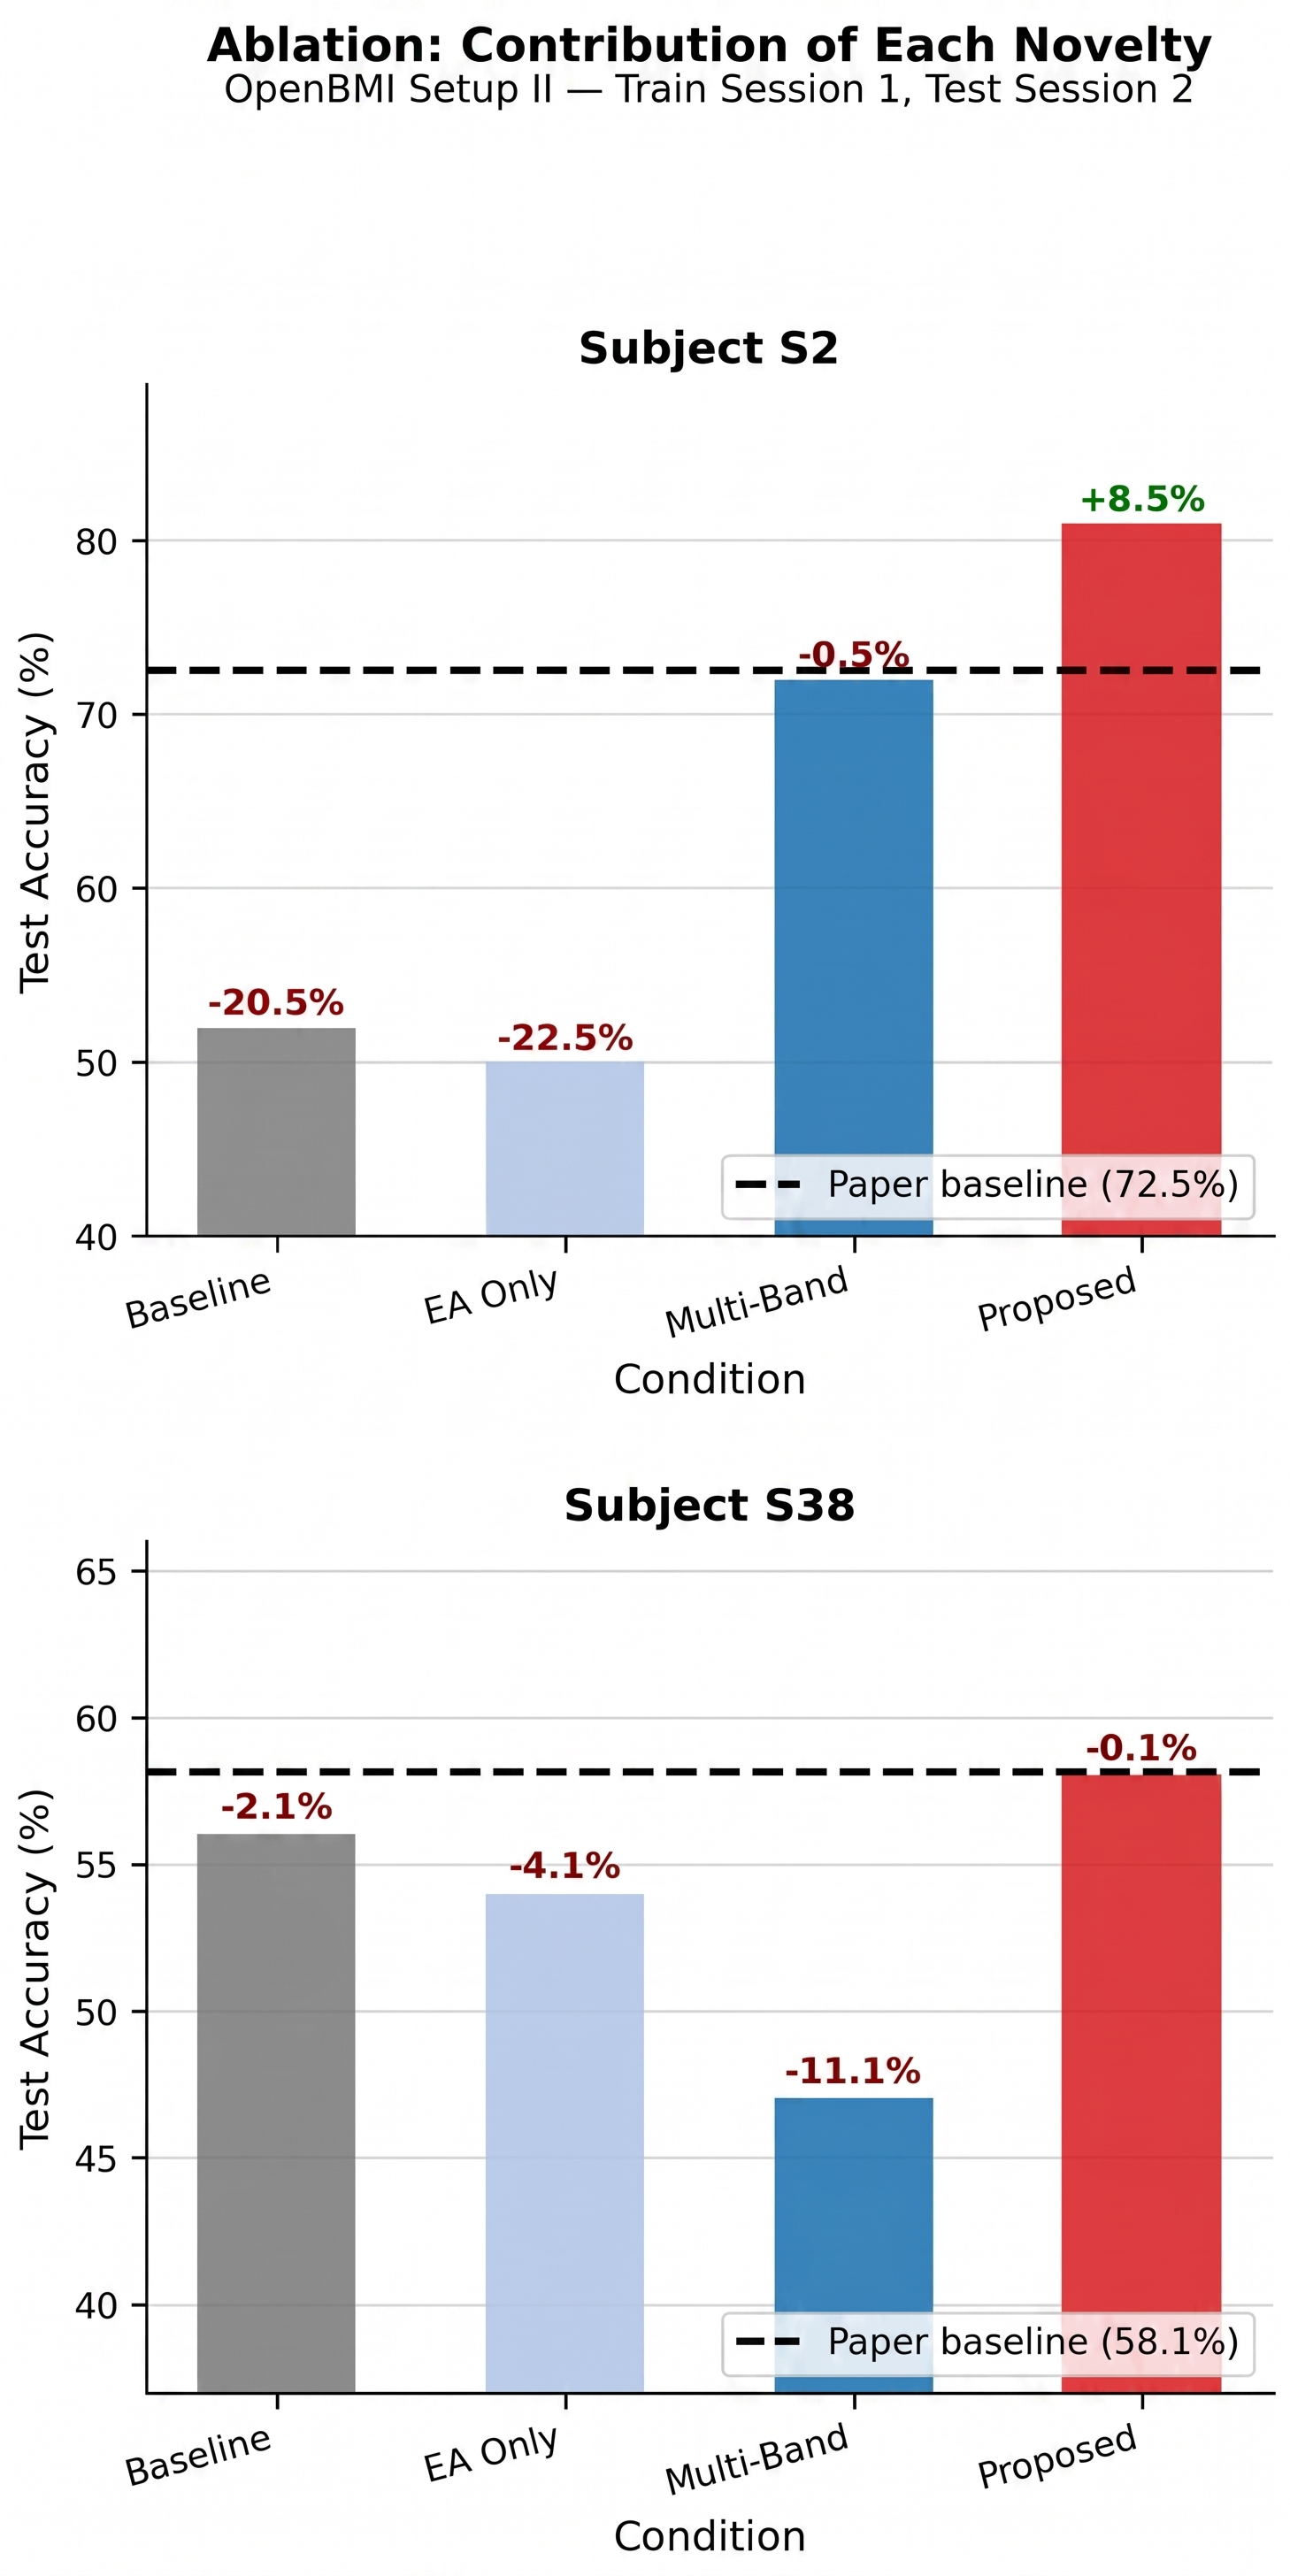
\includegraphics[width=\columnwidth]{exp3_ablation.png}}
\caption{Component ablation on OpenBMI: S2 (Surge Subject) and S38 (Stable-Manifold Subject). Dashed line = SWCNet Setup~II paper baseline per subject.}
\label{fig:openbmi_ablation}
\end{figure}

For S2, the Baseline condition achieves 52.0\%, already 20.5\% below the paper baseline, confirming the raw model is insufficient under distributional shift. EA~Only drops further to 50.0\% ($-22.5$\% vs.\ paper). Multi-Band~Only recovers to 72.0\% ($-0.5$\% vs.\ paper), demonstrating that frequency decomposition alone substantially recovers cross-session performance without alignment. The Proposed model achieves 81.0\% (+8.5\% vs.\ paper), establishing that the synergy of EA and multi-band together is the critical factor: EA corrects the covariance manifold so that multi-band features are extracted from a geometrically consistent representation.

For S38, the CV-Test Dissociation pattern from HGD~S5 is replicated faithfully. Baseline achieves 56.0\% ($-2.1$\% vs.\ paper). EA~Only drops to 54.0\% ($-4.1$\%). Multi-Band~Only collapses to 47.0\% ($-11.1$\%)---an unusually large degradation revealing that the Stable-Manifold boundary condition is more severe at 62 channels: when the spatial manifold is already well-aligned across sessions, the expanded 186-channel input amplifies irrelevant frequency noise rather than isolating discriminative ERD features. The Proposed model recovers to 58.0\% ($-0.1$\% vs.\ paper), showing that EA and multi-band partially cancel each other's negative effects for Stable-Manifold subjects at high electrode density.

\subsubsection*{PSD Analysis: Surge vs Stable-Manifold}

Fig.~\ref{fig:openbmi_psd} presents a six-panel PSD comparison (Broadband, Mu, Beta rows; S2 and S38 columns) for right-hand vs.\ left-hand motor imagery.

\begin{figure}[t]
\centerline{\includegraphics[width=\columnwidth]{exp2_psd_multiband.png}}
\caption{PSD: S2 (Surge Subject) and S38 (Stable-Manifold Subject) across Broadband, Mu, and Beta bands. Solid = Right Hand; Dashed = Left Hand. Shaded = $\pm1$ SD.}
\label{fig:openbmi_psd}
\end{figure}

For S2, the Broadband PSD exhibits a prominent peak near 10~Hz where right-hand and left-hand traces diverge clearly---a classic Mu ERD signature. In the Mu panel, this separation is preserved with reduced variance, confirming that targeted 8--13~Hz filtering isolates the discriminative rhythm while suppressing out-of-band noise. The Beta panel reveals a secondary separation near 15--16~Hz, indicating S2 exhibits both Mu and low-Beta ERD contributions. The multi-band decomposition captures both, enabling the $(3C, 1)$ kernel to weight these complementary frequency views---directly explaining S2's large gain under the Proposed model.

For S38, the Broadband PSD shows much smaller and less structured class separation, with both classes nearly overlapping across 4--40~Hz. In the Mu panel, the class traces remain almost indistinguishable with extensively overlapping variance bands, indicating absent canonical Mu ERD. The Beta panel shows some separation near 15~Hz but with large within-class variance. This attenuated ERD profile---consistent with the Stable-Manifold phenotype on HGD S3, S5, and S9---explains why multi-band expansion fails to improve S38's Setup~II accuracy. Notably, S38's Setup~I accuracy is 99.29\% (Table~\ref{tab:openbmi_combined}), confirming that this subject's MI features are learnable within-session; the failure is purely a consequence of cross-session manifold shift interacting with weak ERD signatures.

Together, S2 and S38 on OpenBMI replicate and extend the Surge vs.\ Stable-Manifold dichotomy first identified on HGD, confirming that this physiological subpopulation structure is a robust cross-dataset phenomenon.

\subsection{Adaptive Screening for Stable-Manifold Subjects}

The cross-dataset analysis surfaces two converging indicators that reliably flag Stable-Manifold Subjects using only Session~1 data: (1) near-ceiling Setup~I accuracy (above approximately 95\%) and (2) an attenuated Mu-band Fisher ratio (below approximately 5.0). When both conditions hold simultaneously, applying EA reduces cross-session accuracy rather than improving it. We therefore propose the following lightweight screening rule for adaptive preprocessing:

\begin{itemize}
    \item Compute Setup~I accuracy and the Mu Fisher ratio from Session~1 data alone.
    \item If Setup~I accuracy $> 95\%$ \textbf{and} Mu Fisher ratio $< 5.0$: apply the original SWCNet without any alignment or multi-band expansion.
    \item Otherwise: apply the full MB-SWCNet pipeline.
\end{itemize}

This rule correctly identifies S5 and S9 on HGD (Frobenius drift $< 100$, Fisher $< 5$) and S38 on OpenBMI as Stable-Manifold candidates, matching the ablation findings without requiring any Session~2 information. The thresholds stated here are derived empirically from the present three datasets; prospective validation on held-out subjects and refinement of the boundaries is left for future work.

\subsection{Cross-Dataset Mechanistic Summary}

The three datasets reveal a consistent and complementary mechanistic picture. On BCIC-IV-2a, all 9 subjects improve under Setup~II, with gains distributed between EA (high-drift subjects) and the fortified ensemble (low-drift subjects). On HGD, EA provides dramatic gains for Surge Subjects but is harmful for Stable-Manifold Subjects---those with naturally stable inter-session manifolds and attenuated ERD signatures. On OpenBMI, the S2 ablation confirms the EA$+$multi-band synergy as the primary driver of large gains for extreme-drift subjects, while S38 replicates the Stable-Manifold boundary condition at 62 channels where multi-band expansion amplifies noise rather than discriminative features. Across all three datasets, the Stable-Manifold Subject phenomenon is associated with two converging indicators: near-ceiling Setup~I accuracy (S35 on OpenBMI = 99.82\%; S3 on HGD = 95.01\%) and attenuated PSD class separation---providing a reliable pre-session screening criterion whose practical implementation is formalized in the adaptive rule above.

% -------------------------------------------------------
\section{Discussion}
% -------------------------------------------------------

\subsection{Electrode-Density Scaling Law}

The most notable pattern in our results is the monotonic scaling of average Setup~II improvement with electrode density: +4.41\% on 22-channel BCIC-IV-2a, +4.35\% on 44-channel HGD, and +8.03\% on 62-channel OpenBMI. This scaling law has a clear mechanistic explanation: as electrode density increases, (1) the raw inter-session covariance shift grows with the dimensionality of the spatial manifold, making EA more impactful for Extreme- and Moderate-Drift Subjects; and (2) higher electrode density provides more spatial resolution for the multi-band expansion to discover subject-specific ERD topographies. On OpenBMI, 186 spatial-frequency channels feed the $(3C, 1)$ spatial kernel, enabling a degree of subject-specific pattern discovery that is simply unavailable at lower channel counts. The super-responders S21 and S36 reaching 100\% cross-session accuracy are the extreme expression of this scaling effect.

It should be noted that the OpenBMI comparison uses 62 channels in MB-SWCNet versus 20 channels in the original SWCNet evaluation. While this limits strict numerical comparability on OpenBMI, the scaling law is supported independently by the BCIC-IV-2a (22 ch) to HGD (44 ch) progression, which uses matched electrode configurations. The OpenBMI result is therefore best interpreted as an upper bound on the benefit achievable with full spatial resolution, and the controlled cross-dataset trend provides the primary evidence for the scaling relationship.

\subsection{The Stable-Manifold Subject Problem and Clinical Implications}

The existence of Stable-Manifold Subjects---approximately 35--40\% of HGD subjects and a similar proportion on OpenBMI---represents a clinically significant finding. These are subjects who achieve high cross-session accuracy without any alignment intervention because their neural topology is naturally consistent across recording days. For these individuals, applying EA introduces mathematical noise by distorting a manifold that did not need correcting. Their PSD profiles showing attenuated Mu/Beta power serve as a complementary indicator: subjects with weak canonical ERD signatures are simultaneously likely to have stable manifolds.

A practical consequence of this finding is that population-level average accuracy improvements understate the benefit for Surge Subjects while masking harm to Stable-Manifold Subjects. Clinical deployment should therefore treat subject classification as a prerequisite step rather than an optional refinement. The two-criterion screening rule proposed in Section~\ref{sec:mechanistic} provides a computationally free mechanism to make this determination from Session~1 data alone, requiring no additional recording or user burden. The optimal model for confirmed Stable-Manifold Subjects remains the original SWCNet~\cite{b1} without preprocessing modifications, reinforcing the value of the base architecture within the broader adaptive pipeline.

\subsection{The CV-Test Dissociation Effect}

A consistent and diagnostically critical pattern across all ablation conditions is that cross-validation accuracy on the training session remains high (95--99\%) regardless of condition, while test accuracy on Session~2 varies dramatically. This CV-Test Dissociation Effect carries two important implications. First, it proves that the primary challenge in Setup~II is not model capacity or label noise on Session~1---the model demonstrably learns the MI task well within a single session. The failure is caused exclusively by distributional shift between sessions. Second, it justifies why we targeted the preprocessing level with EA rather than simply making the neural network larger or deeper: no amount of architectural complexity can overcome a systematic distributional shift that the model never sees during training. EA addresses the root cause directly, before the neural network is involved.

\subsection{Ensemble and Label Smoothing Contributions}

The fortified ensemble pipeline provides consistent secondary benefits beyond EA and multi-band decomposition. The 5-model soft-voting ensemble reduces prediction variance, particularly for subjects near decision boundaries in the 4-class HGD setting and for subjects with low Mu Fisher ratios. Label Smoothing ($\epsilon = 0.1$) prevents overconfident predictions, especially important when the 35-inference ensemble processes subjects with weak MI signatures whose Softmax distributions tend toward degenerate peaks.

\subsection{Computational Overhead}

MB-SWCNet introduces two sources of additional computation relative to SWCNet. Multi-band decomposition triples the effective channel dimension, increasing the parameter count of the spatial convolution by a factor of three. The 5-model ensemble requires five inference passes per trial. EA itself involves a matrix square root of order $\mathcal{O}(C^3)$ per session, which is computationally negligible for $C \leq 62$. The overall training time is therefore approximately three to four times that of SWCNet on equivalent hardware. For time-sensitive or resource-constrained deployment, the ensemble can be reduced to a single model trained on the full training set, accepting a modest accuracy reduction in exchange for single-pass inference latency.

% -------------------------------------------------------
\section{Conclusion}
% -------------------------------------------------------

We have proposed Multi-Band SWCNet (MB-SWCNet), a framework that extends the Space-First convolutional architecture of SWCNet \cite{b1} with two targeted preprocessing novelties---Per-Session Euclidean Alignment and Multi-Band Spatial-Frequency Expansion---and a fortified ensemble training pipeline. Under both Setup~I (single-session) and strict Subject-Dependent Setup~II (cross-session) evaluation protocols, MB-SWCNet achieves consistent improvements over SWCNet \cite{b1} across all three benchmark datasets:

\begin{itemize}
    \item \textbf{BCIC-IV-2a:} Setup~I 99.81\% (+2.39\%); Setup~II 74.00\% (+4.41\%), F1 = 0.7340, improvements on all 9 subjects.
    \item \textbf{High Gamma Dataset:} Setup~I 99.96\% (+7.70\%); Setup~II 86.16\% (+4.35\%), with gains up to +26.50\% on individual subjects.
    \item \textbf{OpenBMI:} Setup~I 99.50\% (+8.68\%) across 54 subjects; Setup~II 65.18\% (+8.03\%), two subjects reach 100\% cross-session accuracy.
\end{itemize}

Beyond numerical improvements, this work makes six key conceptual contributions. First, it establishes Per-Session EA as a principled and computationally lightweight solution to cross-session covariance shift, requiring no labelled target-session data. Second, it demonstrates that the $(3C, 1)$ Space-First kernel acts as a subject-specific frequency selector---mathematically forced by the multi-band input structure to learn optimal cross-band spatial weightings per subject---a mechanism directly supported by the Mu band's 31\% higher Fisher ratio relative to broadband. Third, it introduces the formal \textit{Stable-Manifold Subject} taxonomy, providing the first systematic physiological explanation for when EA is harmful and motivating subject-adaptive preprocessing pipelines. Fourth, it establishes the \textit{CV-Test Dissociation Effect} as the diagnostic proof that Setup~II performance collapse is caused by distributional shift, not model capacity. Fifth, it demonstrates a clear \textit{electrode-density scaling law} in which the benefit of both EA and multi-band expansion compounds with spatial dimensionality, culminating in 100\% cross-session accuracy for extreme-drift subjects on 62-channel OpenBMI. Sixth, it proposes a two-criterion pre-session screening rule that identifies Stable-Manifold Subjects from Session~1 data alone, providing a practical path toward adaptive deployment without additional recording burden.

Future work will focus on: (1) prospective validation of the adaptive screening rule on held-out subject cohorts; (2) extending the evaluation to subject-independent (LOSO) protocols on all three datasets; and (3) investigating adaptive frequency band selection---learning optimal bandpass boundaries per subject rather than relying on fixed physiological priors.

\begin{thebibliography}{00}
\bibitem{b1} K. Singh, N. Singha, G. Jaswal, and S. Bhalaik, ``A Novel CNN With Sliding Window Technique for Enhanced Classification of MI-EEG Sensor Data,'' \textit{IEEE Sensors Journal}, vol. 25, no. 3, pp. 4777--4786, Feb. 2025.
\bibitem{b2} J. van Erp, F. Lotte, and M. Tangermann, ``Brain--computer interfaces: Beyond medical applications,'' \textit{Computer}, vol. 45, no. 4, pp. 26--34, Apr. 2012.
\bibitem{b3} L. F. Nicol\'{a}s-Alonso and J. Gomez-Gil, ``Brain computer interfaces, a review,'' \textit{Sensors}, vol. 12, no. 2, pp. 1211--1279, Jan. 2012.
\bibitem{b4} M. Orban, M. Elsamanty, K. Guo, S. Zhang, and H. Yang, ``A review of brain activity and EEG-based brain--computer interfaces for rehabilitation application,'' \textit{Bioengineering}, vol. 9, no. 12, p. 768, Dec. 2022.
\bibitem{b5} N. Padfield, J. Zabalza, H. Zhao, V. Masero, and J. Ren, ``EEG-based brain--computer interfaces using motor-imagery: Techniques and challenges,'' \textit{Sensors}, vol. 19, no. 6, p. 1423, Mar. 2019.
\bibitem{b6} S. Sakhavi, C. Guan, and S. Yan, ``Learning temporal information for brain--computer interface using convolutional neural networks,'' \textit{IEEE Trans. Neural Netw. Learn. Syst.}, vol. 29, no. 11, pp. 5619--5629, Nov. 2018.
\bibitem{b7} J. Chen, Z. Yu, Z. Gu, and Y. Li, ``Deep temporal--spatial feature learning for motor imagery-based brain--computer interfaces,'' \textit{IEEE Trans. Neural Syst. Rehabil. Eng.}, vol. 28, no. 11, pp. 2356--2366, Nov. 2020.
\bibitem{b8} B. Blankertz, R. Tomioka, S. Lemm, M. Kawanabe, and K.-R. M\"{u}ller, ``Optimizing spatial filters for robust EEG single-trial analysis,'' \textit{IEEE Signal Process. Mag.}, vol. 25, no. 1, pp. 41--56, Jan. 2008.
\bibitem{b9} R. T. Schirrmeister et al., ``Deep learning with convolutional neural networks for EEG decoding and visualization,'' \textit{Human Brain Mapping}, vol. 38, no. 11, pp. 5391--5420, Nov. 2017.
\bibitem{b10} V. J. Lawhern, A. J. Solon, N. R. Waytowich, S. M. Gordon, C. P. Hung, and B. J. Lance, ``EEGNet: A compact convolutional neural network for EEG-based brain--computer interfaces,'' \textit{J. Neural Eng.}, vol. 15, no. 5, Jul. 2018, Art. no. 056013.
\bibitem{b11} P. Wang, A. Jiang, X. Liu, J. Shang, and L. Zhang, ``LSTM-based EEG classification in motor imagery tasks,'' \textit{IEEE Trans. Neural Syst. Rehabil. Eng.}, vol. 26, no. 11, pp. 2086--2095, Nov. 2018.
\bibitem{b12} R. Zhang, Q. Zong, L. Dou, X. Zhao, Y. Tang, and Z. Li, ``Hybrid deep neural network using transfer learning for EEG motor imagery decoding,'' \textit{Biomed. Signal Process. Control}, vol. 63, Jan. 2021, Art. no. 102144.
\bibitem{b13} H. Li, M. Ding, R. Zhang, and C. Xiu, ``Motor imagery EEG classification algorithm based on CNN-LSTM feature fusion network,'' \textit{Biomed. Signal Process. Control}, vol. 72, Feb. 2022, Art. no. 103342.
\bibitem{b14} H. Altaheri, G. Muhammad, and M. Alsulaiman, ``Physics-informed attention temporal convolutional network for EEG-based motor imagery classification,'' \textit{IEEE Trans. Ind. Informat.}, vol. 19, no. 2, pp. 2249--2258, Feb. 2023.
\bibitem{b15} X. Tang, C. Yang, X. Sun, M. Zou, and H. Wang, ``Motor imagery EEG decoding based on multi-scale hybrid networks and feature enhancement,'' \textit{IEEE Trans. Neural Syst. Rehabil. Eng.}, vol. 31, pp. 1208--1218, 2023.
\bibitem{b16} H. He and D. Wu, ``Transfer learning for brain--computer interfaces: A Euclidean space data alignment approach,'' \textit{IEEE Trans. Biomed. Eng.}, vol. 67, no. 2, pp. 399--410, Feb. 2020.
\bibitem{b17} C. Brunner et al., ``BCI competition 2008---Graz data set A,'' Graz University of Technology, 2008.
\bibitem{b18} M.-H. Lee et al., ``EEG dataset and OpenBMI toolbox for three BCI paradigms: An investigation into BCI illiteracy,'' \textit{GigaScience}, vol. 8, no. 5, May 2019, Art. no. giz002.
\bibitem{b19} S. Ioffe and C. Szegedy, ``Batch normalization: Accelerating deep network training by reducing internal covariate shift,'' \textit{arXiv:1502.03167}, 2015.
\bibitem{b20} G. E. Hinton, N. Srivastava, A. Krizhevsky, I. Sutskever, and R. R. Salakhutdinov, ``Improving neural networks by preventing co-adaptation of feature detectors,'' \textit{arXiv:1207.0580}, 2012.
\end{thebibliography}

\end{document}